\documentclass[x11names]{article}
\usepackage{tikz}
\usepackage{pgfplots}
\usepackage{xcolor}
\usepackage{svg}
\usepackage{amsmath}
\usepackage{array}
\usepackage[skins]{tcolorbox}
\usepackage[version=4]{mhchem}
\usepackage[a4paper, total={6in, 10in}]{geometry}
%\usepackage{fourier}
\usepackage{xymtex}
\usepackage{textcomp}
\usepackage{eurosym}
\usepackage{mathrsfs}
\usepackage{float}
\usepackage{pst-all}
\usepackage{pst-3dplot}
\usepackage{leftindex}
\usepackage{verbatim}
\usepackage{import}
\usepackage{xifthen}
\usepackage{pdfpages}
\usepackage{transparent}
\usepackage{import}
\usepackage{pdfpages}
\usepackage{transparent}
\usepackage{amssymb}
\usepackage{mathrsfs}
\usepackage{hyperref}
\usepackage{darkmode}
\usepackage{cancel}
\usepackage{siunitx}
\usepackage{tikz-3dplot}

\usepackage{physics}
\usepackage{tikz}
\usepackage[outline]{contour} % glow around text
\usetikzlibrary{patterns,decorations.pathmorphing}
\usetikzlibrary{decorations.markings}
\usetikzlibrary{arrows.meta}
\usetikzlibrary{calc}
\tikzset{>=latex}
\contourlength{1.1pt}

\colorlet{mydarkblue}{blue!40!black}
\colorlet{myblue}{blue!30}
\colorlet{myred}{red!65!black}
\colorlet{vcol}{green!45!black}
\colorlet{watercol}{blue!80!cyan!10!white}
\colorlet{darkwatercol}{blue!80!cyan!80!black!30!white}
\tikzstyle{water}=[draw=mydarkblue,top color=watercol!90,bottom color=watercol!90!black,middle color=watercol!50,shading angle=0]
\tikzstyle{horizontal water}=[water,
top color=watercol!90!black!90,bottom color=watercol!90!black!90,middle color=watercol!80,shading angle=0]
\tikzstyle{dark water}=[draw=blue!20!black,top color=darkwatercol,bottom color=darkwatercol!80!black,middle color=darkwatercol!40,shading angle=0]
\tikzstyle{vvec}=[->,very thick,vcol,line cap=round]
\tikzstyle{force}=[->,myred,very thick,line cap=round]
\tikzstyle{width}=[{Latex[length=3,width=3]}-{Latex[length=3,width=3]}]

\colorlet{watercol}{blue!80!cyan!10!white}
\colorlet{darkwatercol}{blue!80!cyan!20!white}
\colorlet{metalcol}{blue!40!black!10!white}
\tikzstyle{force}=[->,myred,very thick,line cap=round]
\tikzstyle{vvec}=[->,very thick,vcol,line cap=round]
\tikzstyle{ground}=[preaction={fill,top color=black!10,bottom color=black!5,shading angle=20},
fill,pattern=north east lines,draw=none,minimum width=0.3,minimum height=0.6]
\tikzstyle{mass}=[line width=0.6,red!30!black,fill=red!40!black!10,rounded corners=1,
top color=red!40!black!20,bottom color=red!40!black!10,shading angle=20]
\tikzstyle{rope}=[brown!70!black,line width=1.2,line cap=round] %very thick
\tikzstyle{piston}=[blue!50!black,top color=blue!30,bottom color=blue!50,middle color=blue!20,shading angle=0]
\tikzstyle{water}=[draw=mydarkblue,top color=watercol!90,bottom color=watercol!90!black,shading angle=5]
\tikzstyle{vertical water}=[water,
top color=watercol!90!black!90,bottom color=watercol!90!black!90,middle color=watercol!80,shading angle=90]
\tikzstyle{dark water}=[draw=mydarkblue,top color=darkwatercol,bottom color=darkwatercol!80!black,shading angle=5]
\tikzstyle{metal}=[draw=metalcol!20!black,top color=metalcol,bottom color=metalcol!90!black,shading angle=10]
\tikzstyle{width}=[{Latex[length=3,width=3]}-{Latex[length=3,width=3]}]
\tikzstyle{force}=[->,myred,thick,line cap=round]
\tikzstyle{Fproj}=[force,myred!40]
\newcommand{\vbF}{\vb{F}}
\tikzstyle{rope}=[brown!20!black,double=brown!70!black,double distance=1,line width=0.3] %very thick
%\def\rope#1{ \draw[black,line width=2.3] #1; \draw[rope] #1; }
\def\tick#1#2{\draw[thick] (#1)++(#2:0.1) --++ (#2-180:0.2)}


% TIKZ settings
\usetikzlibrary{arrows,arrows.meta}
\tikzset{>=latex}
\colorlet{vcol}{green!60!black}
\tikzstyle{vvec}=[-{Latex[length=4,width=3]},thick,vcol,line cap=round]
\tikzstyle{myarr}=[-{Latex[length=3,width=2]}]
\tikzstyle{mydoublearr}=[{Latex[length=3,width=2]}-{Latex[length=3,width=2]}]
\tikzset{
	pics/eye/.style={
		code={
			\draw (#1-180:0.5) to[out=#1,in=#1-240,looseness=0.9] (#1-90:0.25)
			(#1-180:0.5) to[out=#1,in=#1-130,looseness=0.9] (#1-270:0.25);
			\clip (#1-180:0.47) to[out=#1,in=#1-240,looseness=0.9] (#1-90:0.24) --
			(#1-270:0.242) to[out=#1-130,in=#1,looseness=0.9] cycle;
			\draw[very thin,top color=white,bottom color=red!60!black!20,shading angle=#1-120]
			(#1-180:0.48) circle(0.45);
			\fill[brown!30!black,rotate=#1-180]
			(0.07,0) ellipse({0.05} and 0.12);
			\fill[black,rotate=#1-180]
			(0.05,0) ellipse({0.03} and 0.06);
	}},
	pics/eye/.default=180
}
% REST
\def\R{1.5}      % radius
\def\N{5}        % number of wave fronts
\def\lam{\R/\N}  % wavelength
\def\angmin{30}  % min. angle velocity arrow
\def\angmax{330} % min. angle velocity arrow
\def\waves#1{
	\foreach \i in {1,...,\N}{
		\draw[blue,thick] ({-(\i-0.25)*#1*\lam},0) circle ({\lam*(\i-0.25)});
	}
	\foreach \a in {\angmin,90,150,210,270,\angmax}{
		\draw[myarr,vcol] ({-(\N-0.25)*#1*\lam},0)++(\a:\R-0.50*\lam) --++ (\a:\lam);
	}
	\fill[red] (0,0) circle (0.06);
}

% svg + latex
\usepackage{import}
\usepackage{xifthen}
\usepackage{pdfpages}
\usepackage{transparent}

\newcommand{\incfig}[1]{%
	\def\svgwidth{\columnwidth}
	\import{./imgs/}{#1.pdf_tex}
}

%\enabledarkmode
\definecolor{yblue}{RGB}{224, 245, 255} 
\definecolor{yred}{RGB}{234, 222, 255}
\definecolor{yorange}{RGB}{255, 102, 0}

% box
\newtcolorbox{es}[2][]{%
	enhanced,colback=white,colframe=black,coltitle=black,
	sharp corners,boxrule=0.4pt,
	fonttitle=\itshape,
	attach boxed title to top left={yshift=-0.5\baselineskip-0.4pt,xshift=2mm},
	boxed title style={tile,size=minimal,left=0.5mm,right=0.5mm,
		colback=white,before upper=\strut},
	title=#2,#1
}

% definizioni
\newtcolorbox{blues}[2][]{%
	enhanced,colback=yblue,colframe=black,coltitle=black,
	sharp corners,boxrule=0.4pt,
	attach boxed title to top left={yshift=-0.5\baselineskip-0.4pt,xshift=2mm},
	boxed title style={tile,size=minimal,left=0.5mm,right=0.5mm,
		colback=yblue,before upper=\strut},
	title=#2,#1
}

% teoremi
\newtcolorbox{redes}[2][]{%
	enhanced,colback=yred,colframe=black,coltitle=black,
	sharp corners,boxrule=0.4pt,
	fonttitle=\itshape,
	attach boxed title to top left={yshift=-0.5\baselineskip-0.4pt,xshift=2mm},
	boxed title style={tile,size=minimal,left=0.5mm,right=0.5mm,
		colback=yred,before upper=\strut},
	title=#2,#1
}


% comandi per quadrati dimostrazioni
\newcommand*{\QEDA}{\null\nobreak\hfill\ensuremath{\blacksquare}}%
\newcommand*{\QEDB}{\null\nobreak\hfill\ensuremath{\square}}%

\newcommand{\viola}[1]{\colorbox{yred}{$\displaystyle #1$}}


%% regole
\renewcommand*\contentsname{Indice}
\setcounter{tocdepth}{3}
\setcounter{secnumdepth}{2}
\pgfplotsset{compat=1.15}

\usetikzlibrary{arrows}


\title{Geometria e Algebra lineare}
\author{Federico Cesari}
\date{}



%% DOCUMENTO


\begin{document}
	
\begin{titlepage}
	\begin{center}
		\vspace*{1cm}
		
		\textbf{\LARGE Relazione di laboratorio - Pendolo semplice}
		
		\vspace{0.3cm}
		\large \textit{Misura del periodo di un pendolo semplice} \\
		
		\vspace{0.5cm}
		\Large Federico Cesari \\
		
		\small 1096759 
		\vspace{0.2cm}
		
		\small Gruppo 5
		
		
		\vspace{3cm}
		\begin{center}
			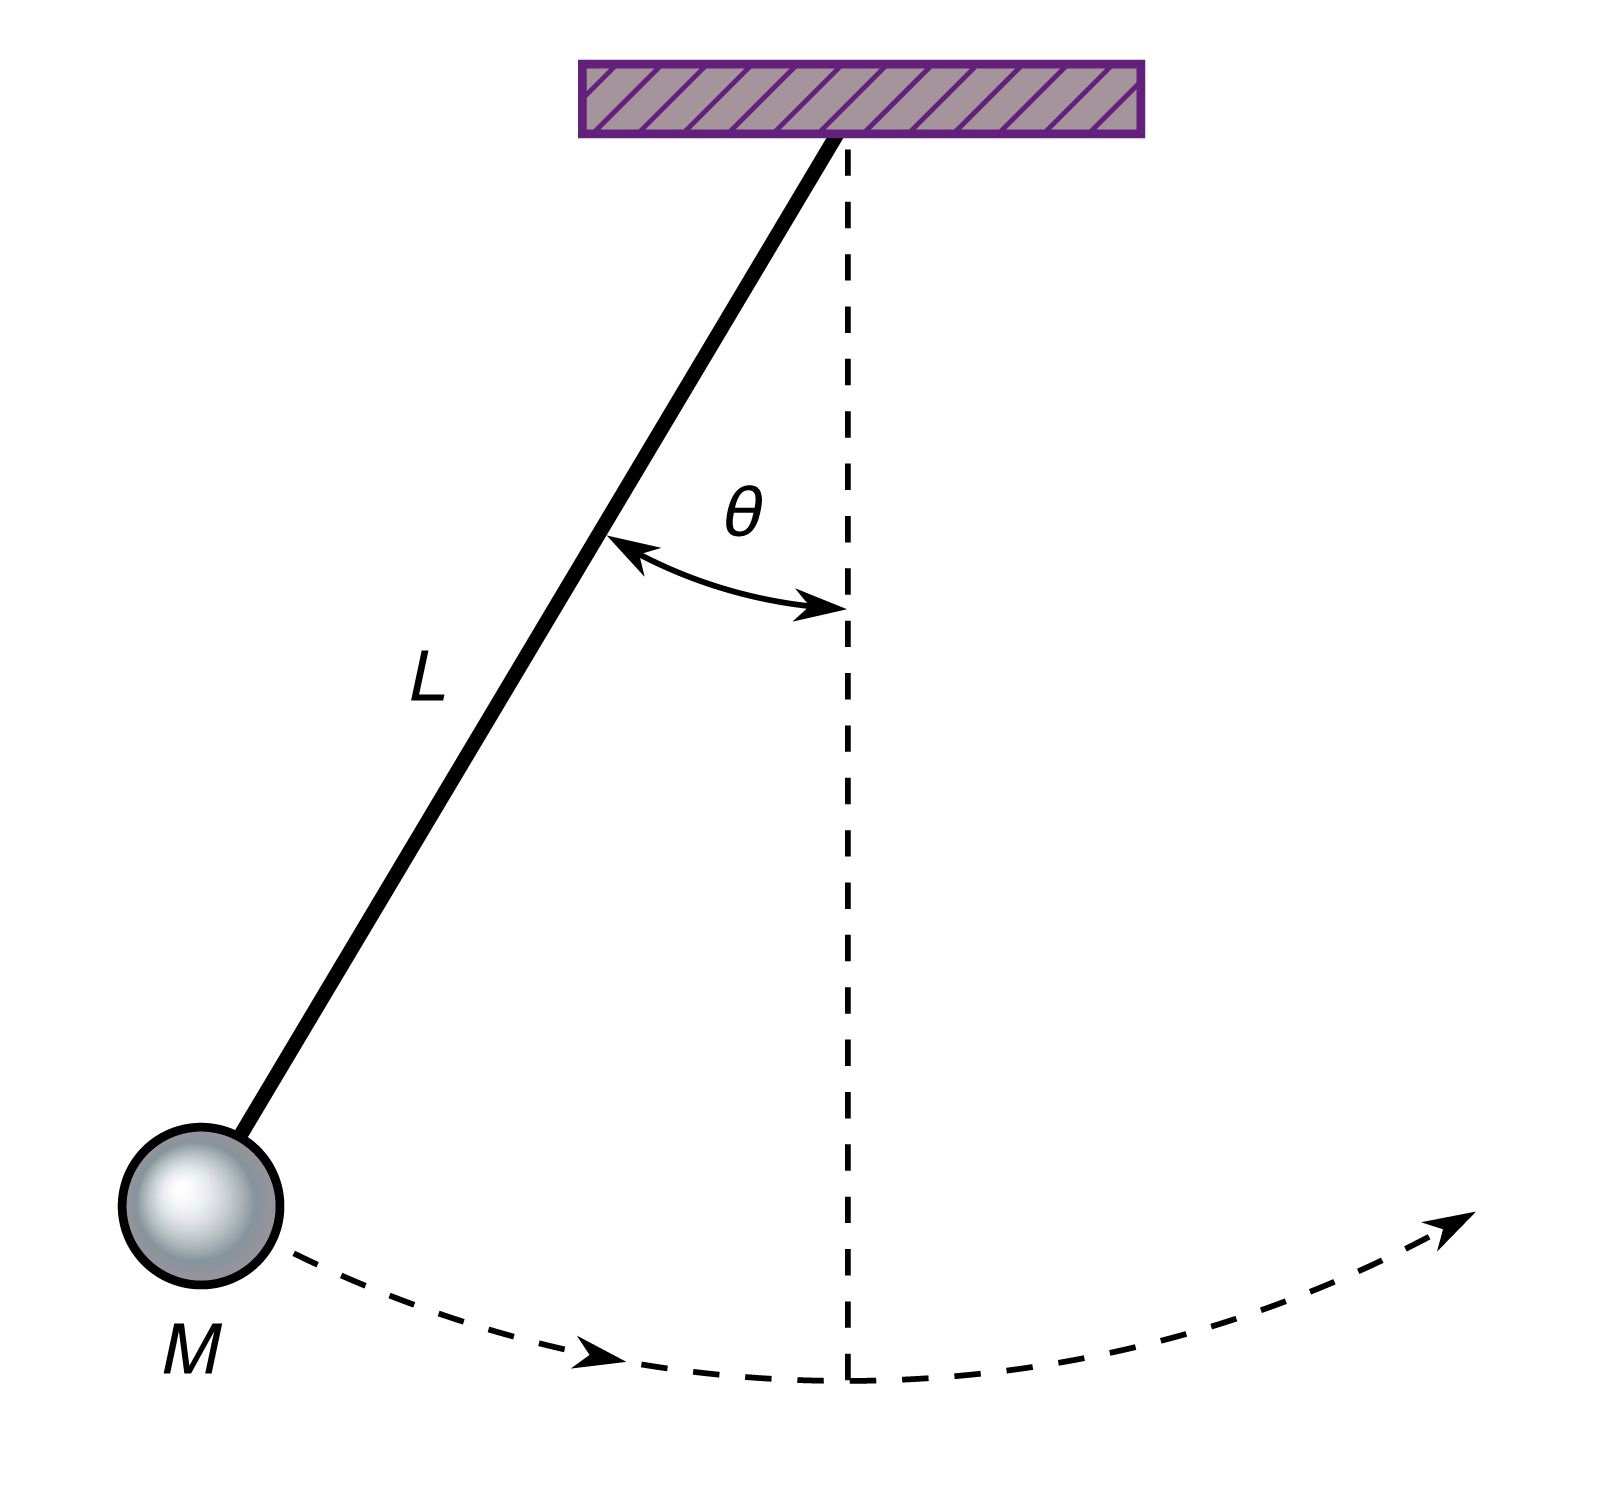
\includegraphics[scale=0.1]{IMG_0200.jpeg}	
		\end{center}
		
		
		
		\vfill
		
		
		
		corso A\\
		Università degli studi di Torino, Torino\\
		4 aprile 2024\\
		
		
	\end{center}
\end{titlepage}
\tableofcontents
\newpage
	
\section{Onde meccaniche}
	Se in casi come il pendolo o un corpo attaccato ad una molla l'oscillazione è \textbf{macroscopica} perché tutto il sistema oscilla, in corpi continui elastici possono prodursi moti oscillatori locali, provocati in una zona specifica del corpo. Questa oscillazione indotta localmente si \textbf{propaga nel mezzo} con una certa velocità costituendo così un'\textbf{onda}.
	
	\begin{center}
		\fboxsep11pt
		\colorbox{yblue}{\begin{minipage}{5.75in}
				\begin{blues}{Definizione: \textbf{Onda}}
					Un'onda è una perturbazione locale impulsiva e periodica che si porpaga in un mezzo (corpo continuo ed elastico) con una certa velocità \(v\). Nel caso unidimensionale parliamo di \textbf{onda piana} \(\xi(x,t)\) la cui deformazione è costante in tutti i punti con stessa \(x\)
				\end{blues}
		\end{minipage}}
	\end{center}
	
	Per descrivere l'andamento di un'onda possiamo: \textbf{fissare un istante \(t\)} e osservare la deformazione su tutto lo spazio \(x\), come se fosse una foto dell'onda; oppure \textbf{fissare un punto dello spazio \(x\)} e osservare al variare del tempo come varia la forma dell'onda, come se fosse un filmato.
	
	\begin{center}
		\textcolor{red}{inserire grafici}
	\end{center}
	
	Vediamo ora come possiamo scrivere l'equazione che descrive la perturbazione in funzione della posizione \(\mathbf{x}\) e del tempo \(\mathbf{t}\): per farlo serviamoci di un sistema di riferimento \(\mathbf{O}\) solidale con l'istante \(t=0\) e un sistema di riferimento \(\mathbf{O'}\) solidale con lo spostamento dell'onda che viaggia a velocità \(v\).
	
	Possiamo quindi descrivere la posizione l'andamento di un'onda piana tramite una funzione del tipo
	
	\[ 
	\begin{cases} 
		x' = x\pm vt \\ \xi' = \xi 
	\end{cases} 
	\quad \Rightarrow \quad \xi(x,t) = \mathbf{f(x \pm vt)}
	\]
	
	Una funzione del tipo \(\mathbf{f(x \pm vt)}\) soddisfa l'equazione differenziale detta \textbf{equazione delle onde} o \textbf{equazione di d'Alembert}:
	
	\[ 
	\nabla^2_\xi- \frac{1}{v^2} \frac{\partial^2\xi}{\partial t^2} = 0 \quad \Rightarrow \quad \boxed{\frac{\partial^2\xi}{\partial x^2} = \frac{1}{v^2}\frac{\partial^2\xi}{\partial t^2}}
	\]
	
	\begin{es}{dimostrazione}
		\[ 
		\mathbf{z = x - vt} \quad \Longleftrightarrow \quad \boxed{\frac{\partial z}{\partial x} = 1}   \quad \quad \boxed{\frac{\partial z}{\partial t} = -v}  \quad \Longleftrightarrow \quad  \mathbf{f = f(z)}
		\]
		
		\[ 
		\textcolor{blue}{\frac{\partial^2 f}{\partial x^2} =} \frac{\partial}{\partial x}\left(\frac{\partial f}{\partial x}\right) =\frac{\partial}{\partial x}\left(\frac{\partial f}{\partial z}\frac{\partial z}{\partial x}\right)  \textcolor{blue}{=\frac{\partial^2 f}{\partial z^2}}
		\]
		\[ 
		\textcolor{red}{\frac{\partial^2 f}{\partial t^2} =} \frac{\partial}{\partial t}\left(\frac{\partial f}{\partial t}\right) =\frac{\partial}{\partial t}\left(\frac{\partial f}{\partial z}\textcolor{orange}{\frac{\partial z}{\partial t}}\right) =\textcolor{cyan}{\frac{\partial}{\partial t}}\left(\textcolor{orange}{-v}\frac{\partial f}{\partial z}\right) = \textcolor{cyan}{-v\frac{\partial }{\partial z}}\left(\textcolor{orange}{-v}\frac{\partial f}{\partial z}\right) \textcolor{red}{=v^2\frac{\partial^2 f}{\partial z^2}}
		\]
		\[ 
	    \frac{\partial^2\xi}{\partial x^2} = \frac{1}{v^2}\frac{\partial^2\xi}{\partial t^2}
		\]
		\newline
		Il passaggio più ambiguo è quello evidenziato in \textcolor{cyan}{ciano}, in cui viene cambiata variabile di derivazione da \(t\) a \(z\). Trattando una funzione qualsiasi, la derivata di qualsiasi funzione rispetto a \(t\) è uguale a \(-v\) derivata rispetto a z (\(-v\) rappresenta il \(dz\) che va a moltiplicare). 
	\end{es}	
	
	\noindent
	Notare che l'equazione delle onde è soddisfatta solo per funzioni che hanno come argomento combinazioni lineari di \(x\) e \(t\) (\(\xi(x \pm vt)\)); è perciò \textbf{l'argomento che importa e non la funzione in sè}. Una combinazione lineare di soluzioni è ancora soluzione dell'equazione, la soluzione generale ha forma
	\[ 
	G(x,t) = f(x-vt) + g(x+vt)
	\]
	


\newpage
\subsection{Onde in una sbarra solida}
	Prendiamo una sbarra solida  e supponiamo di sollecitare  il tratto iniziale applicando una \textbf{forza impulsiva}. Analiziamo un segmento di lunghezza \(dx\): su di esso agiscono la forza elastica \(\vec{F}(x,t)\)  esercitata dagli elementi a sinistra del segmento e la forza elastica \(-\vec{F}(x + dx,t)\) di verso opposto esercitata dagli elementi a destra.

	\begin{center}
		\textcolor{red}{inserire grafici}
	\end{center}
	
	\noindent
	Alla cessazione dello stimolo (\(t'\)) agiscono le forze elastiche e si ha che la lunghezza dell'elemento passa da \(dx\) a 
	\[ 
	(x + dx) + \xi(x+dx,t') \textcolor{gray}{-x - \xi(x,t') } \quad = \quad dx + d\xi
	\]
	Per quanto riguarda le forze invece vale la legge di Hooke secondo la quale
	\[ 
	\textbf{Legge di Hooke} \qquad	F(x) = ES\frac{\partial\xi}{\partial x}
	\]
	Possiamo quindi scrivere la legge del moto con accelerazione \(a = \partial^2 \xi / \partial t^2\):
	\[ 
	\textbf{Risultante} \qquad	dF = \frac{\partial F}{\partial x}dx = \frac{\partial}{\partial x}\left(ES\frac{\partial\xi}{\partial x}\right)dx = ES\frac{\partial^2\xi}{\partial x^2} \mathbf{= dm a} = dm \frac{\partial^2 \xi}{\partial t^2}
	\]
	esprimendo la massa come \(dm = \rho S dx\) si ottiene l'equazione delle onde di d'Alembert dove il coefficiente del termine a destra gioca il ruolo di \(1/v^2\), da questo possiamo scrivere la velocità di propagazione dell'onda:
	\[ 
	E\textcolor{orange}{S}\frac{\partial^2\xi}{\partial x^2}\textcolor{red}{dx} = \rho \textcolor{orange}{S} \textcolor{red}{dx} \frac{\partial^2 \xi}{\partial t^2}
	\]
	
	
	\begin{equation}
		\viola{\frac{\partial^2\xi}{\partial x^2} = \frac{\rho}{E} \frac{\partial^2 \xi}{\partial t^2} \qquad \qquad v = \sqrt{\frac{E}{\rho}}}
	\end{equation}
	
	
	\noindent
	Inoltre oltre allo spostamento \(\xi(x,t)\) si propaga anche la forza \(F(x,t)\). Ciò è verificabile riutilizzando l'epressione della forza nella Legge di Hooke (derivandola prima rispetto a \(t\) e poi rispetto a \(x\)) e ricordando il Teorema di Schwartz, secondo il quale in una derivata mista non dipende dall'ordine di derivazione:
	
	\[ 
	\textcolor{red}{\frac{\partial^2F}{\partial t^2}} = \frac{\partial^2}{\partial t^2} \left(ES\frac{\partial\xi}{\partial x}\right) = \frac{\partial}{\partial x} \left(ES\textcolor{blue}{\frac{\partial^2\xi}{\partial t^2}}\right) = \frac{\partial}{\partial x} \left(ES\textcolor{blue}{v^2\frac{\partial^2\xi}{\partial x^2}}\right) 
	\]
	
	\[ 
	\textcolor{purple}{\frac{\partial^2F}{\partial x^2}} = \frac{\partial^2}{\partial x^2} \left(ES\frac{\partial\xi}{\partial x}\right) = \frac{\partial}{\partial x} \left(ES\frac{\partial^2\xi}{\partial x^2}\right)
	\]
	
	\[ 
	\begin{cases}
		\frac{\partial}{\partial x} \left(ES\frac{\partial^2\xi}{\partial x^2}\right) = \textcolor{purple}{\frac{\partial^2F}{\partial x^2}} \\
		\frac{\partial}{\partial x} \left(ESv^2\frac{\partial^2\xi}{\partial x^2}\right)  =  \textcolor{red}{\frac{\partial^2F}{\partial t^2}}
	\end{cases} \to 
	\begin{cases}
		\frac{\partial}{\partial x} \left(ES\frac{\partial^2\xi}{\partial x^2}\right) = \textcolor{purple}{\frac{\partial^2F}{\partial x^2}} \\
		\frac{\partial}{\partial x} \left(ES\frac{\partial^2\xi}{\partial x^2}\right)  = \frac{1}{v^2} \textcolor{red}{\frac{\partial^2F}{\partial t^2}}
	\end{cases}
	\]
	

	\begin{equation}
		\viola{\frac{\partial^2F}{\partial x^2} = \frac{1}{v^2} \frac{\partial^2 F}{\partial t^2} \qquad \qquad v = \sqrt{\frac{E}{\rho}}}
	\end{equation}

	
	\begin{center}
		\fboxsep11pt
		\colorbox{yblue}{\begin{minipage}{5.75in}
				\begin{blues}{Definizione: onde lognitudinali}
					Quando, come in questo caso, sia lo spostamento \(\xi(x\pm vt)\) sia la forza \(F(x\pm vt)\), campi che descrivono le onde che si propagano lungo l'asse x, sono paralleli alla direzione in cu si propaga la perturbazione, l'onda viene chiamata \textbf{onda longitudinale}.
				\end{blues}
		\end{minipage}}
	\end{center}
	
\newpage
\subsection{Onde in una corda tesa}
	Quando si sposta rapidamente in direzione trasversale l'estremo di una corda tesa (con un estremo fisso) vediamo la perturbazione che si propaga lungo la corda da un estremo all'altro. Supponiamo di spostare leggermente la corda dalla sua posizione di equilibrio e andiamo a studiare le tensioni che agiscono su un segmento di corda \(\mathbf{dl}\). Per piccoli angoli \(\alpha\) e \(\alpha'\) possiamo introdurre le seguenti approssimazioni:
	
	\[ 
	\cos{\alpha} = 1 \quad \cos{\alpha'} = 1 \qquad \qquad \sin{\alpha} = \tan{\alpha} \quad \sin{\alpha'} = \tan{\alpha'}
	\]
	\[ 
	\boxed{\tan\alpha = \frac{\partial \xi}{\partial x} = S(x,t)}
	\]
	
	\begin{center}
		\textcolor{red}{inserire grafici}
	\end{center}
	
	
	\[ 
	dF_x = T(\cos\alpha' - \cos\alpha ) = 0 
	\]
	\[ 
	 dF_y = T(\sin\alpha' - \sin\alpha ) = T(\tan\alpha' - \tan\alpha ) = T\left[S(x+dx,t) - S(x)\right] = TdS = T\frac{\partial S}{\partial x}dx = T\frac{\partial}{\partial x}\left(\frac{\partial \xi}{\partial x}\right)dx = T\frac{\partial^2 \xi}{\partial x^2}dx
	\]
	
	\[ 
	\textbf{Risultante} \qquad	dF =  T\frac{\partial^2 \xi}{\partial x^2}dx  \mathbf{= dm a} = dm \frac{\partial^2 \xi}{\partial t^2} 
	\]
	esprimendo la massa come \(dm = \mu dx\) si ottiene l'equazione delle onde di d'Alembert dove il coefficiente del termine a destra gioca il ruolo di \(1/v^2\), da questo possiamo scrivere la velocità di propagazione dell'onda:
	\[ 
	T\frac{\partial^2\xi}{\partial x^2}\textcolor{red}{dx} = \mu \textcolor{red}{dx} \frac{\partial^2 \xi}{\partial t^2}
	\]

	\begin{equation}\label{corda}
		\viola{	\frac{\partial^2\xi}{\partial x^2} = \frac{\mu}{T} \frac{\partial^2 \xi}{\partial t^2} \qquad \qquad v = \sqrt{\frac{T}{\mu}}}
	\end{equation}
	
	\begin{center}
		\fboxsep11pt
		\colorbox{yblue}{\begin{minipage}{5.75in}
				\begin{blues}{Definizione: onde trasversali}
					Quando, come in questo caso, le particelle del mezzo attraversato subiscono spostamenti in direzione perpendicolare alla direzione in cui si propaga l'onda l'onda viene chiamata \textbf{onda trasversale}.
				\end{blues}
		\end{minipage}}
	\end{center}
	
\newpage
\subsection{Onde nei gas}
	Se per i solidi la deformazione dipende dal modulo di Young secondo la legge \(\frac{\Delta L}{L} = \frac{1}{E}\sigma\), nel caso dei gas la variazione relativa di volume segue la legge
	\[ 
	\frac{\Delta V}{V} = -\frac{1}{\beta} \Delta p
	\] \\
	
	\noindent
	Supponiamo di avere del gas imperturbato (\(\rho_0, p_0\)) bloccato da due pistoni. Fornendo un impulso di pressione tramite i pistoni provociamo una compressione adiacente con una \textbf{conseguenti variazione di densità di massa}.
	
	\[
	\rho = \rho + d\rho \qquad p = p_0 + dp
	\]
	
	\subsubsection{Densità}
	Considero un elemnto di gas di massa \(dm = \rho_0S(dx)\) che a seguito della perturbazione subisce uno spostamento che lo porta a stare tra
	\[
	x + \xi(x,t') \quad \text{ e } \quad x + dx + \xi(x + dx,t')
	\]
	Così la sua dimensione diventa
	\[
	x + dx + \xi(x + dx,t') \textcolor{gray}{-x - \xi(x,t')} = dx + \xi(x + dx,t')- \xi(x,t') = dx + \frac{\partial \xi}{\partial x}dx = dx\left(1 + \frac{\partial \xi}{\partial x}\right)
	\]
	A partire da questa nuova espressione della "larghezza" dell'elemnto infinitesimo posso scrivere l'espressione della densità dopo la compressione:
	\[
	\rho(x,t) = \frac{dm}{dV} = \frac{\rho_0 \textcolor{red}{S (dx)}}{\textcolor{red}{Sdx}\left(1 + \frac{\partial \xi}{\partial x}\right)} = \rho_0\left(1 + \frac{\partial \xi}{\partial x}\right)^{-1}
	\]
	Ora andremo ad applicare una semplificazione bizzarra. Se la deformazione specifica $|\varepsilon| = \left|\frac{\partial \xi}{\partial x}\right|<< 1$, allora si può applicare la formula del binomio:
	\[
	\left(1 + \varepsilon\right)^{-n} = 1 - n\varepsilon + \textcolor{gray}{\frac{n(n+1)}{2!}\varepsilon^2\dots}
	\]
	Quindi posso scrivere la densità come
	\[
	\rho(x,t) \approx \rho_0\left(1 - \frac{\partial \xi}{\partial x}\right)
	\]
	da cui la variazione
	\begin{equation} \label{rho}
	d\rho(x,t) = \rho(x,t) - \rho_0 = - \rho_0\frac{\partial \xi}{\partial x}
	\end{equation}
	in cui il segno meno indica ce se il volumetto è compresso la densità aumenta, mentre se si espande la densità diminuisce.
	
	\subsubsection{Pressione}
	Ad una variazione di densità corrisponde una variazione di pressione secondo la legge
	\[
	\beta = \rho_0\frac{dp}{d\rho} \quad \to \quad dp(x,t) = p(x,t) - p_0 = \beta\frac{d\rho}{\rho_0}
	\]
	da cui derivo che la pressione è 
	\[
	p(x,t) = \beta\frac{d\rho}{\rho_0} +  p_0 
	\]
	Sostituendo l'espressione della densità trovata prima nella \ref{rho} scrivo
	\begin{equation}\label{1press}
	\viola{p(x,t)} = \beta\frac{- \rho_0\frac{\partial \xi}{\partial x}}{\rho_0} +  p_0 \viola{=p_0 - \beta\frac{\partial \xi}{\partial x}}
	\end{equation}
	\subsubsection{Forza}
	La variazione di pressione causa un movimento del gas e la risultante su $dm$ è 
	\begin{align*}
	-dF = F(x,t') - F(x+dx.t') =& S\left[p(x,t') - p(x+dx,t')\right] \\
							   =& S(dp) \\
							   =& -S\frac{\partial p}{\partial x}dx \\
							   =& -S\frac{\partial}{\partial x}\left(p_0 - \beta\frac{\partial \xi}{\partial x}\right)dx \\
							   =& S\beta\frac{\partial^2\xi}{\partial x^2}dx
	\end{align*}
	
	\[ 
	\textbf{Risultante} \qquad	-dF = S\beta\frac{\partial^2\xi}{\partial x^2}dx  \mathbf{= dm a} = \rho_0 S(dx) \frac{\partial^2 \xi}{\partial t^2} 
	\]
	
	\begin{equation} \label{gas}
		\viola{\frac{\partial^2\xi}{\partial x^2} = \frac{\rho_0}{\beta} \frac{\partial^2 \xi}{\partial t^2} \qquad \qquad v = \sqrt{\frac{\beta}{\rho_0}}}
	\end{equation}
	
	Lungo la colonna di gas si propagano anche un'onda i pressione e una perturbazione di densità del gas, tuttue con la stessa velocitù data da \ref{gas}.
	
	\subsubsection{Modulo di compressibilità adiabatica}
	Nel caso di trasformazioni adiabatiche vale (come dimostreremo più avanti) l'uguaglianza
	\[
	pV^\lambda = \text{costante}
	\]
	dalla quale, sviluppando il differenziale si possono trovare alcune caratteristiche di \(\beta\) in condizioni adiabatiche:
	\[
	d\left(pV^\gamma\right) = V^\gamma (dp) + \gamma p V^{(\gamma - 1)}dV \boldsymbol{= 0}
	\]
	\[ 
	\to \quad  V^\gamma (dp) = \gamma p V^{(\gamma - 1)}(dV) \quad \to \quad \frac{\textcolor{red}{V^\gamma} (dp)}{p\textcolor{red}{V^\gamma}} = \frac{\gamma \textcolor{red}{p} V^{(\gamma - 1)}(dV)}{\textcolor{red}{p}V^\gamma}
	\]
	Dalla quale otteniamo (confrontata con l'espressione precedente di \(\beta\))
	\[ 
	\frac{dp}{p} = \gamma\frac{dV}{V} 
	\]
	\[ 
	\frac{dV}{V} = \frac{1}{p\gamma}dp  \qquad \qquad \frac{\Delta V}{V} = -\frac{1}{\beta} \Delta p
	\]
	Da cui si ottiene la nuova espressione di \(\beta\)
	
	
	\begin{equation}
		\viola{\beta = \gamma p}
	\end{equation}
	
	\begin{es}{calcolo velocità del suono}
		Se assimiliamo l'aria ad un gas perfetto biatomico (\(\gamma = 7/5\)) dai risultati ottenuti fin'ora si trova che:
		\[ 
		v = \sqrt{\frac{\beta}{\rho_0}} = \sqrt{\frac{\gamma p_0}{\rho_0}} = \sqrt{\frac{(7/5)\cdot 1.01325\cdot 10^5}{1.29}} = 331.6 \frac{m}{s}
		\]
		Il risultato ottenuto è in accordo (3\%) con quello misurato, possiamo quindi dedurre che l'aprossimazione adiabatica è una bona approssimazione.
	\end{es}
	
	
\newpage
\section{Onde piane armoniche}
Un tipo molto importante di onda piana è l'\textbf{onda armonica} la cui forma si scrive

\[ 
\xi(x,t) = \xi_0 \sin\left(\boldsymbol{k}x \mp \boldsymbol{\omega} t + \boldsymbol{\delta}\right)
\]
dove \(k\) è il \textbf{numero d'onde}.
\begin{center}
	\textcolor{red}{inserire grafici}
\end{center}

\noindent
\paragraph{Periodo spaziale} Fissato un tempo \(t=t_0\), definiamo la lunghezza d'onda \(\lambda\) come la periodicità spaziale dell'onda. Essendo \(\lambda\) lo spazio tra due creste d'onda possiamo calcolarla come \(\lambda = x_2 - x_1 = 2\pi / k\), da cui si deduce che \(k\) è uguale al numero di lunghezze d'onda in un intervallo spaziale pari a \(2\pi\) metri.

In generale il periodo spaziale può essere espresso tramite \(\lambda\) o \(k\).

\begin{center}
	\fboxsep11pt
	\colorbox{yblue}{\begin{minipage}{5.75in}
			\begin{blues}{Lunghezza d'onda \(\lambda\)}
				La lungheza d'onda è lo spazio percorso dalla perturbaione nell'intervallo di tempo di un periodo \(T\).
				\[ 
				\lambda = \frac{2\pi}{k} = vT
				\]
			\end{blues}
	\end{minipage}}
\end{center}

\paragraph{Periodo temporale} Fissato unpunto nello spazio \(x=x_0\), definiamo il periodo \(T = t_2-t_2\)

\[ T = \frac{2\pi}{\omega}\] 
come l'intervallo temporale tra due istanti nei quali l'onda, essendo armonica, assume lo stesso valore.

Sapendo che la pulsazione è la velocità dell'onda nel percorrere un giro (\(2\pi\)), i due periodi dono legati dalla relazione
\[ 
\lambda = vT
\]
Quindi possiamo esprimere il periodo temporale tramite \(T\), \(f\), \(\omega\).\\

\noindent
Tutte le espressioni della funzione d'onda sono:

\[ 
\xi(x,t) = \xi_0 \sin\left(kx \mp \omega t + \delta\right) \qquad \xi(x,t) = \xi_0 \sin\left[ 2\pi\left(\frac{x}{\lambda} \mp \frac{t}{T}\right) + \delta\right]  \qquad \xi_0\sin\left[\frac{2\pi}{\lambda}\left(x \mp vt\right) + \delta \right]
\]
	
	
	\newpage
	\subsection{Propagazione dell'energia in una barra solida}
	La propagazione di un campo che descrive in'onda è sempre accompagnato da una propagazione di energia. Osserviamo prima il fenomeno del flusso di energia legato alla propagazione di un'onda piana armonica in una barra solida andando a calcolare la potenzia media e l'energia per untià di volume ad essa associata.\\
	
	\begin{center}
		\textcolor{red}{inserire grafici}
	\end{center}
	
	\noindent
	Per prima cosa mettiamo in evidenza le equazioni che entrano in gioco:
	\[ 
	\textbf{Onda:} \quad \xi(x,t) = \xi_0\sin\left(kx - \omega t\right)
	\]
	\[ 
	\textbf{Forza:} \quad F = -ES\frac{\partial\xi}{\partial x}
	\]
	L'espressione della potenza è 
	
	\begin{align*}
		\mathcal{P} =& \vec{F} \cdot \vec{u} \\
					=& -ES\frac{\partial\xi}{\partial x}\frac{\partial\xi}{\partial t} \\
					=& -ES\left[k\xi_0\cos\left(kx -\omega t\right)\right]\left[-\omega \xi_0\cos\left(kx -\omega t\right)\right] \\
					=& ESk\omega \xi_0^2\cos^2\left(kx-\omega t\right)
	\end{align*}
	La potenza quindi è una cosinusoide traslata in alto di una sua ampiezza (con avvallamenti tangenti all'asse orizzontale). la potenza media è espirmibile come la retta che interseca la cosinusoide alla quota pari a metà la sua ampiezza; poi ricordandoci che
	
	\[ 
	\boxed{v = \sqrt{E/\rho} \qquad E = v^2 \rho} \qquad \boxed{k = \frac{\omega}{v}}
	\]
	
	\begin{align*}
		\mathcal{P}_m =& \frac{1}{2} ESk\omega \xi_0^2  \\
			=& \frac{1}{2} (v^2 \rho)S\left(\frac{\omega}{v}\right) \omega\xi_0^2 
	\end{align*}
	
	\begin{equation}
		\viola{\mathcal{P}_m = \frac{1}{2}\rho \omega^2 \xi^2 S v}
	\end{equation}
	
	
	\subsubsection{Energia per unità di volume}
	Considero l'elemento infinitesimo di massa \(dm = \rho dV = \rho S dx\) descrive un moto armonico con 
	\[ 
	\textbf{Posizione:} \quad \xi(x,t) = \xi_0\sin\left(kx - \omega t\right) 
	\]
	\[ 
	\textbf{Velocità} \quad v(x,t)= \frac{\partial\xi}{\partial t} = \omega \xi_0\cos\left(kx - \omega t\right) 
	\]
	Quindi l'energia meccanica risulta pari all'energia cinetica massima assunto dall'elemento \(dm\), che si trova utilizzando la velocità massima \(v_{\text{max}} = \omega \xi_0\):
	
	\[ 
	dU = \frac{1}{2}(dm)v_{\text{max}}^2 = \frac{1}{2}\rho S (dx)\omega^2 \xi_0^2 = \frac{1}{2}\rho (dV)\omega^2 \xi_0^2
	\]
	Chiamiamo \textbf{densità di energia per unità di volume} il valore 
	\[
	\mathcal{W} = \frac{dU}{dV} = \frac{1}{2}\rho \omega^2\xi_0^2
	\]
	con la quale possiamo esprimere la potenza media come 
	
	\begin{equation}
		\viola{\mathcal{P}_m = \mathcal{W}S v}
	\end{equation}

	
	\subsubsection{Intensità dell'onda}
	Definiamo l'intensità di un'onda come  \textbf{potenza media per unità di superficie}, quindi
	
	\[
	I = \frac{\mathcal{P}_m}{S} = \frac{1}{2}\rho\omega^2\xi_0^2v
	\]
	
	\subsection{Propagazione dell'energia in una corda tesa}
	Studiamo ora lo stesso fenomeno ma in una corda tesa. La situazione è simile con la differenza che l'onda ora è trasversale.
	
	\begin{center}
		\textcolor{red}{inserire grafici}
	\end{center}
	
	\noindent
	Per prima cosa mettiamo in evidenza le equazioni che entrano in gioco:
	\[ 
	\textbf{Onda:} \quad \xi(x,t) = \xi_0\sin\left(kx - \omega t\right)
	\]
	\[ 
	\textbf{Forza:} \quad F = T
	\]
	L'espressione della potenza è 
	
	\begin{align*}
		\mathcal{P} =& \vec{F} \cdot \vec{u} \\
		=& T\frac{\partial\xi}{\partial t}\cos{\left(\frac{\pi}{2} + \alpha\right)} \qquad  \cos{\left(\frac{\pi}{2} + \alpha\right)} = \sin{\alpha} \approx \tan\alpha = \frac{\partial\xi}{\partial x} \\
		= & T\frac{\partial\xi}{\partial t}\frac{\partial\xi}{\partial x} \\
		=& Tk\omega \xi_0^2\cos^2\left(kx-\omega t\right)
	\end{align*}
	Trovo la potenza media come prima esprimendo \(k\) e \(T\) come
	\[ 
	\boxed{v = \sqrt{T/\mu} \qquad T = v^2 \mu} \qquad \boxed{k = \frac{\omega}{v}}
	\]
	
	\begin{equation}
		\viola{\mathcal{P}_m = \frac{1}{2}\mu\omega^2\xi^2v}
	\end{equation}
	
	
	\subsubsection{Energia per unità di lunghezza}
	Considero l'elemento infinitesimo di massa \(dm = \mu dx \) descrive un moto armonico con 
	\[ 
	\textbf{Posizione:} \quad \xi(x,t) = \xi_0\sin\left(kx - \omega t\right) 
	\]
	\[ 
	\textbf{Velocità} \quad v(x,t)= \frac{\partial\xi}{\partial t} = \omega \xi_0\cos\left(kx - \omega t\right) 
	\]
	Quindi l'energia meccanica risulta pari all'energia cinetica massima assunto dall'elemento \(dm\), che si trova utilizzando la velocità massima \(v_{\text{max}} = \omega \xi_0\):
	
	\[ 
	dU = \frac{1}{2}(dm)v_{\text{max}}^2 = \frac{1}{2}\mu(dx)\omega^2 \xi_0^2 
	\]
	Chiamiamo \textbf{densità di energia per unità di lunghezza} il valore 
	\[
	\mathcal{W} = \frac{dU}{dx} = \frac{1}{2}\mu \omega^2\xi_0^2
	\]
	con la quale possiamo esprimere la potenza media come 
	
	\begin{equation}
		\viola{\mathcal{P}_m = \mathcal{W} v}
	\end{equation}

	\subsection{Onde sonore}\label{Onde Sonore}
	Consideriamo ora delle onde sonore come onde di spostamento sempre accompagnate da onde di pressione:
	\[ 
	\textbf{Spostamento: }\quad \xi = \xi _0\sin(kx-\omega t)
	\]
	\[ 
	\textbf{Pressione: }\quad dp = -\beta \frac{\partial\xi}{\partial x}
	\]
	\subsubsection{Pressione}
	L'espressione della pressione era stata ricavata nel capitolo sulle onde nei gas (\ref{1press})
	\[ 
	p(x,t) = p_0 -\beta \frac{\partial \xi }{\partial x} \quad \to \quad dp(x,t) = p(x,t) - p_0 = -\beta \frac{\partial \xi }{\partial x}
	\]
	Sviluppando la derivata parziale, e ricordando alcune equivalenze
	\[ 
	\boxed{v = \sqrt{\frac{\beta}{\rho_0}} \to  \beta = v^2\rho_0} \qquad \boxed{k = \frac{\omega }{v}}
	\]
	troviamo
	\begin{align*}
		dp =& -\textcolor{red}{\beta} \textcolor{blue}{k} \xi_0 \cos\left(kx-\omega t\right) \\
		   =& \textcolor{red}{v^2 \rho_0}\textcolor{blue}{\frac{\omega }{v}} \cos\left(kx-\omega t\right) \\
		   =& \boldsymbol{\rho_0 v \omega  \xi_0}  \cos\left(kx-\omega t\right) \\ 
		   =& \boldsymbol{\Delta p_{\text{max}}} \sin\left(kx -\omega t - \pi /2\right) \\
	\end{align*}
	Le onde di pressione sono quindi in ritardo di \(\pi /2\).
	
	\subsubsection{Potenza}
	\[ 
	\mathcal{P} = \overrightarrow{F}\cdot \vec{v} = (dp)S v = -\beta \frac{\partial\xi}{\partial x} S \frac{\partial\xi}{\partial t}
	\]
	\begin{align*}
		\mathcal{P} &= \beta k \xi_0 \cos\left(kx- \omega t\right) S \omega  \xi_0 \cos\left(kx- \omega t\right)\\
					&= v^2\rho_0 \frac{\omega}{v} \xi_0 \cos\left(kx- \omega t\right) S \omega \xi_0 \cos\left(kx- \omega t\right)\\
					&=  \rho_0 v \omega ^2 S \xi_0^2 \cos^2\left(kx- \omega t\right) 
	\end{align*}
	Si ottiene quindi una potenza media pari a metà la sua ampiezza
	\[ 
	\mathcal{P}_m = \frac{1}{2} \rho_0 v \omega ^2 S \xi_0^2
	\]
	\subsubsection{Intensità}
	Ricordando che l'intensità è la potenza per unità di superficie:
	\[ 
	I = \frac{\mathcal{P}_m }{S} =   \frac{1}{2} \rho_0 v \omega ^2 \xi_0^2
	\]
	Riconosciamo che \(\Delta p_{\text{max}} = \rho_0 v \omega  \xi_0\) e che quindi possiamo scrivere l'intensità come
	\begin{equation}\label{intensita_fono}
		\viola{I = \frac{(\rho_0 v \omega  \xi_0)^2}{2\rho_0 v} = \frac{\Delta p_{\text{max}}^2}{2\rho_0 v}}
	\end{equation}
	
	
	\subsection{Fonometria}
	Per essere messo in movimento il timpano ha bisogno di un'intensità minima che chiamiamo \textbf{soglia di udibilità}. Il limite superiore invece è chiamata \textbf{soglia del dolore} e rappresenta l'intensità sopra alla quale si percepisce una sensazione dolorosa. Entrambe vengono espresse o in funzione della frequenza o in funzione della lunghezza d'onda (\(\lambda=v/f\)); si ha quindi che le frequenze all'interno delle due soglie sono
	\[ 
		\SI{20}{\hertz} < f < \SI{20000}{\hertz}
	\]
	\[ 
		\SI{17.15}{\m} < \lambda < \SI{1.715}{\cm}
	\]
	La\textbf{ soglia minima} convenzionale dell'udibilità è l'intensità \(I_0 = 10^{-12}\SI{}{\watt/\m^2}\) alla frequenza  \(f = 10^3\SI{}{\hertz}\). A questa si possono associare la corrispondente onda di pressione e ampiezza delle oscillazioni:
	\[ 
		\Delta p_{\text{max}} = \sqrt{2\rho_0 v I_0} = 2.97 \cdot 10^{-5} \SI{}{\pascal}
	\]
	e poiché  \(\Delta p_{\text{max}} = \rho_0 v \textcolor{red}{\omega } \xi_0\)
	\[ 
		\xi_0 = \frac{\Delta p_{\text{max}}}{\textcolor{red}{2\pi f}\rho_0 v} = 1.07 \cdot 10^{-11}\SI{}{\m}
	\]
	
	Alla soglia del dolore invece si ottengono 
	
	\[ 
	\Delta p_{\text{max}} = \sqrt{2\rho_0 v I_0} = 29.7 \SI{}{\pascal}
	\]
	\[ 
	\xi_0 = \frac{\Delta p_{\text{max}}}{2\pi f\rho_0 v} = 1.07 \cdot 10^{-5}\SI{}{\m}
	\]
	In sintesi: l'orecchio umano si estendi su
	\begin{itemize}
		\item \textbf{3} ordini di grandezza in \textbf{frequenza}: \(0 - 10^3 \SI{}{\hertz}\)
		\item \textbf{12} ordini di grandezza in \textbf{intensità}: \(1 - 10^12 \SI{}{\watt/\m^2}\)
		\item \textbf{6} ordini di grandezza in \textbf{ampiezza di oscillazione}: \(10^{-11} - 10^{-5} \SI{}{\m}\)
	\end{itemize}
	
	
	
	
	
	
	\subsubsection{Livello sonoro}
	Presa una certa intensità \(I\) si definisce un \textbf{livello sonoro} \(L\) rispetto a \(I_0\). Il livello sonoro è una valutazione logaritmica relativa di intensità e si esprime in decibel (\(\SI{}{\decibel}\)).
	
	Al livello sonoro associamo delle curve isofoniche, ovvero il luogo dei punti in cui si percepisce la stessa sensazione uditiva \(S\). 
	
	\begin{equation}\label{livello sonoro}
		\viola{L = 10\log_{10}{\frac{I}{I_0}}}
	\end{equation}
	Vediamo come il livello sonoro risulta essere particolarmente pratico poiché \(L = 0\) con \(I_0\) per \(f=1000\SI{}{\hertz}\), quindi vale 0 alla soglia di udibilità; e vale \(\boldsymbol{120}\) con \(\boldsymbol{I/I_0 = 10^{12}}\) alla soglia del dolore.
	
	\begin{es}{Attenzione}
		Il valore d'intensità \(I_0\) \textbf{dipende dalla frequenza}. Per questo anche il livello sonoro \(L\) non dipende tanto da \(I_0\) quanto più dalla frequenza. 
		
		Le curve isofoniche infatti non descrivono eguale intensità \(I\) ma eguale rapporto \(I/I_0\), che dipende dalla frequenza. Possiamo dire che \(S\) è una grandezza \textit{fisiologica} e \(L\) una grandezza fisica.
	\end{es}
	Secondo la \textbf{legge psicofisica di Fechner e Weber}
	\[ 
	S = kB = k10\log_10{\frac{I}{I_0}} = k'\log_10{\frac{I}{I_0}}
	\]
	quindi
	\begin{equation}
		S_2 - S_1 = k'\log_10{\frac{I_2}{I_1}}
	\end{equation}
	la sensazione sonora è proporzionale al logaritmo del rapporto tra le intensità che hanno prodotto le sensazioni
	
	
	\newpage
	\subsection{Onde in più dimensioni}	
	Prima di tutto definiamo \textbf{fronte d'onda} la superfici su cui in un certo istante la fase dell'onda è costante (\(\phi = kx -\omega t\)). 

	Per le onde piane il fronte d'onda è un piano che si sposta con velocità \(v\) dell'onda. Per caratterizzare la direzione di propagazione dell'onda introduciamo il \textbf{vettore di propagazione} \(\vec{k}\) con \(k = 2\pi/\lambda\) e verso uguale a quello di \(\vec{v}\) e il vettore posizione \(\vec{r}\) che individua la posizione di un punto P su un certo fronte d'onda. Con queste informazioni possiamo riscrivere la funzione d'onda come
	\[ 
	\xi(r,t) = \xi_0 \sin\left(\vec{k}\cdot \vec{r}- \omega t\right) 
	\]
	In un sistema di tre coordinate l'equazione generale delle onde ammette altre soluzioni che rappresentano \textbf{onde sferiche} e \textbf{onde cilindriche}: 
	\[ 
	\nabla^2\xi (x,y,z,t) = \frac{1}{v^2}\frac{\partial^2\xi (x,y,z,t)}{\partial t^2}
	\]
	\subsubsection{Onde elastiche in una membrana tesa}
	Consideriamo una membrana piana tesa con tensione \(T\). Supponiamo di spostare leggermente la membrana dalla sua posizione di equilibrio e andiamo a studioare le tensioni che agiscono su un'area \(dxdy\). 
	
	Il ragionamento è uguale a quello fatto per la corda tesa, in questo caso però la tensione si distribuisce su tutto il lato \(d*\) e diventa \(T(d*)\):
	
	\begin{center}
		\textcolor{red}{inserire grafici}
	\end{center}
	
	\[ 
	dF_x(x,y,z,t) = T(dx)\frac{\partial^2 \xi(x,y,t)}{\partial y^2}dy = T\frac{\partial^2\xi(x,y,t)}{\partial y^2}dxdy
	\]
	\[ 
	dF_y(x,y,z,t) = T\frac{\partial^2 \xi(x,y,t)}{\partial x^2}dx = T(dy)\frac{\partial^2\xi(x,y,t)}{\partial x^2}dxdy 
	\]
	
	\[ 
	\textbf{Risultante} \qquad	dF = T\left(\frac{\partial^2\xi(x,y,t)}{\partial y^2} + \frac{\partial^2\xi(x,y,t)}{\partial x^2}\right)dxdy \mathbf{=(dm)a = }  \rho_s(dxdy)\frac{\partial^2\xi(x,y,t)}{\partial t^2}
	\]
	esprimendo la massa come \(dm = \rho_s (dxdy)\) si ottiene l'equazione delle onde di d'Alembert dove il coefficiente del termine a destra gioca il ruolo di \(1/v^2\), da questo possiamo scrivere la velocità di propagazione dell'onda:
	
	\[ 
	T\left(\frac{\partial^2\xi(x,y,t)}{\partial y^2} + \frac{\partial^2\xi(x,y,t)}{\partial x^2}\right)\textcolor{red}{dxdy} = \rho_s(\textcolor{red}{dxdy})\frac{\partial^2\xi(x,y,t)}{\partial t^2}
	\]
	
	
	\begin{equation}
		\viola{\frac{\partial^2\xi(x,y,t)}{\partial y^2} + \frac{\partial^2\xi(x,y,t)}{\partial x^2} = \frac{\rho_s}{T}\frac{\partial^2\xi(x,y,t)}{\partial t^2} \qquad v = \sqrt{\frac{T}{\rho_s}}}
	\end{equation}

	
	
	
	\subsubsection{Onde sferiche}
	Se il mezzo è \textit{isotropo} è quindi la velocità di propagazione è uguale in tutte le direzioni, la funzoine d'\textbf{onda sferica armonica} è \(\xi(r,t) = A(r)\sin\left(kr -\omega t\right)\) dove \(r\) è la distanza dalla sorgfente e \(A(r)\) è l'ampiezza funzione di \(r\). \\
	

	\begin{figure}[ht]
		\centering
		\scalebox{.7}{\incfig{sfera}}
		\caption{Onde sferiche}
		\label{fig:Onde sferiche}
	\end{figure}
	
	\noindent
	Diciamo che la nostra sorgente emetta un'onda di intensità \(I(r) = CA^2(r)\) dove \(C\) è una costante dipendente dal mezzo. In un'onda sferica la \textbf{potenza media} trasmessa attraverso la superficie sferica \(S = 4\pi r^2\) deve risultare \textbf{costante} ad ogni valore di \(r\):
	
	\[ 
	\mathcal{P}_m = \textcolor{blue}{I}S = \text{cost.}
	\] 
	
	\[ 
	\mathcal{P}_m = \textcolor{blue}{CA^2}4\pi r^2 = \text{cost.}
	\]
	
	\[ 
	A(r) = \sqrt{\frac{\mathcal{P}_m}{4\pi r^2}} = \frac{1}{2r}\sqrt{\frac{\mathcal{P}_m}{\pi}}
	\]

	\noindent
	Risulta quindi che l'ampiezza è inversamente proporzionale alla distanza \(r\), come la pressione, e quindi può essere scritta come \(A = \xi_0 /r\).
	\begin{equation}
		\viola{\xi(r,t) = \frac{\xi_0}{r}\sin\left(kr -\omega t\right)}
	\end{equation}
	
	\subsubsection{Intensità}
	Supponendo che le onde in questione siano onde sonore, andando quindi ad utilizzare le espressioni di pressione della sezione \ref{Onde Sonore} e andando a sostituire ogni \(\xi_0\) con \(\xi_0/r\) si ottiene la seguente espressione dell'intensità:
	
	\[ 
	I(r) = \frac{\mathcal{P}_m}{S} = \frac{1}{2} \rho_0 v \omega ^2 \frac{\xi_0^2}{r^2}
	\]
	
	\subsection{Onde cilindriche}
	


	\newpage
	\subsection{Assorbimento dell'energia}
	Come abbiamo visto l'intensità di un'onda non rimane costante ma decresce al propagarsi dell'onda (nelle onde sferiche più rapidamente, nelle cilindriche meno...). Questo comportamento viene attribuito ad un \textbf{assorbimento di energia} dovuto a fenomeni di attrito interno. Studiando il fenomeno su uno spessore \(dx\) si ha un'aattenuazione che può essere considerata proporzionale all'intensità in \(x\) e allo spessore \(dx\).
	
	\[ 
 	dI = -\boldsymbol{\alpha} I(x)dx
	\]
	
	dove \(\alpha\) è il \textbf{coefficiente di assorbimento}.
	
	\[ 
	\int_{I_0}^{I} \frac{dI}{I} = -\alpha\int_{0}^{x} dx 
	\]
	\begin{equation}
 		\viola{I(x) = I_0e^{-\alpha x}}
	\end{equation}
	Quindi la decrescità dell'intensità è esponenziale. Definiamo la distanza \(x_0 = \frac{1}{\alpha}\) detta \textbf{lunghezza di assorbimento} la distanza tra due punti tali che \(I(x_1)/I(x_2) = \frac{1}{e}\).\\
	
	\noindent
	Abbiamo appurato precedentemente che l'ampiezza dell'onda è direttamente proporzionale a \(\sqrt{I}\)
	
	\[ 
	I = CA^2 \quad \to \quad A = \sqrt{\frac{I}{C}} = \sqrt{\frac{I_0e^{-\alpha x}}{C}}
	\]
	quindi la funzione d'onda in un mezzo che assorbe energia è:
	
	\[ 
	\textbf{Onde piane:}\qquad \xi = \left(\frac{I_0e^{-\alpha x}}{C}\right)^{\frac{1}{2}} \sin\left(kx-\omega t\right) \quad = \quad \xi_0 \left(I_0e^{-\alpha x/2}\right)^{\frac{1}{2}}\sin\left(kx-\omega t\right)
	\]
	\[ 
	\textbf{Onde sferiche:}\qquad \xi = \frac{\left(\frac{I_0e^{-\alpha x}}{C}\right)^{\frac{1}{2}}}{r} \sin\left(kx-\omega t\right) \quad = \quad \xi_0 \frac{\left(I_0e^{-\alpha x/2}\right)^{\frac{1}{2}}}{r}\sin\left(kx-\omega t\right)
	\]
	\[ 
	\textbf{Onde cilindriche:}\qquad \xi = \frac{\left(\frac{I_0e^{-\alpha x}}{C}\right)^{\frac{1}{2}}}{\sqrt{r}} \sin\left(kx-\omega t\right) \quad = \quad \xi_0 \frac{\left(I_0e^{-\alpha x/2}\right)^{\frac{1}{2}}}{\sqrt{r}}\sin\left(kx-\omega t\right)
	\]
	
	\newpage
	\subsection{Pacchetti d'onde}
	Fino ad ora abbiamo considerato onde armoniche di lunghezza e durata infinita. Tutte le sorgenti emettono onde attraverso processi di durata finita, quindi, nella realtà, un'onda ha una propria durata e estensione spaziale.\\
	
	\noindent
	Considerato un pacchetto di lughezza \(\Delta x\) e durata \(\Delta t\), tali che \(\Delta x = v\Delta t\). Il pacchetto è poi caratterizzato da \(N\) oscillazioni tali che
	
	\[ 
\Delta x  =N \lambda \qquad \Delta t = NT 
	\]
	ed esprimiamo il numero di onde \(k\) e la pulsazione \(\omega\) come
	
	\[ 
	k = \frac{2\pi}{\lambda}= \frac{2\pi N}{\Delta x} \qquad \omega = \frac{2\pi}{T} = \frac{2\pi N}{\Delta t}
	\]
	
	\begin{center}
		\textcolor{red}{inserire grafici}
	\end{center}
	Se ammettiamo (come nella figura) che N non sia fisso ma abbia una acerta indeterminazione che esprimiamo come \(\Delta N = 1\), possiamo trovare altre espressioni per \(k\) e \(\omega\):
	
	\[ 
	\boxed{\Delta k = \frac{2\pi}{\Delta x}} \qquad \boxed{ \Delta\omega = \frac{2\pi}{\Delta t}} \qquad \boxed{\Delta f = \frac{1}{\Delta t}}
	\]
	
	\[ 
	\viola{\Delta k \Delta x = 2\pi} \qquad \viola{\Delta \omega \Delta t = 2\pi} \qquad \viola{\Delta f \Delta t = 1}
	\]
	Queste osservazioni mettono i vevidenza la sostanziale differenza tra onda e pacchetto d'onda: mentre la prima ha una lunghezza d'onda \(\lambda\)  e una frequenza \(f\) ben definite che la descrivono completamente, nel secondo è presente una \textbf{banda di frequenze} e un \textbf{intervallo di numeri d'onda}
	\[ 
	\Delta f = \frac{1}{\boldsymbol{\Delta t}} \qquad \Delta k = \frac{2\pi}{\boldsymbol{\Delta x}}
	\]
	Da quest'ultime espressioni notiamo che al crescere di \(\Delta x\) e \(\Delta t\) minori risultano queste bande, infatti la limite per \(\Delta x,\Delta t \to \infty\) troviamo l'onda armonica. Se andiamo a considerare \textbf{brevi durate e piccole lunghezze} nel pacchetto sono contenute bande di lunghezze d'onda e frequenze distribuite significatibamente nell'intorno di \(\lambda\) \(f\).
	
		\subsubsection{Velocità di fase e velocità di gruppo}
		Poiché diversi segmenti d'onda contenuti in un pacchetto possono avere frequenze diverse, la velocità del pacchetto non può essere identificata con quella delle componenti. Tuttavia è essenziale identificare la velocità del pacchetto perché il fenomeno fisico è rappresentato proprio dal pacchetto ed è la sua velocità quella con cui si propaga l'\textbf{energia} dell'onda.     
		
		Andiamo quindi a distinguere la \textbf{velocità di fase}, quella con cui si muovono le singole componenti dell'onda, e \textbf{velocità di gruppo}. 
		La velocità dell'onda dipende dalla frequenza quando la propagazione avviene in un \textbf{mezzo dispersivo} come può avvenire per onde sulla superficie di un liquido o onde elettromagnetiche in mezzi materiali o in cavità conduttrici.\\
		
		\noindent
		Mostriamo un esempio di velocità di gruppo nel caso di un pacchetto con solo due onde armoniche:
		
		\[ 
		\xi(x,t) = \xi_0\sin\left(k_1x -\omega_1 t\right) + \xi_0\sin\left(k_2x -\omega_2 t\right)
		\]
		\[ 
		\textcolor{gray}{\textit{prostaferesi: } \quad \sin\alpha + \sin\beta = 2\sin\left(\frac{\alpha + \beta}{2}\right)\cos\left(\frac{\alpha - \beta}{2}\right)}
		\]
		\[ 
		\xi(x,t) = 2\xi_0\sin\left(\frac{(k_1 + k_2)x - (\omega_1 + \omega_2)t}{2}\right) \cos\left(\frac{(k_1 - k_2)x + (\omega_2 - \omega_1)t}{2}\right)
		\]
		Definiti \(k_m,\omega _m\) e \(\Delta k,\Delta\omega\)
		\[ 
		\boxed{k_m = \frac{k_1 + k_2}{2}} \qquad \boxed{\omega _m = \frac{\omega _1 + \omega _2}{2}} \qquad \boxed{\Delta k=\frac{k_1 - k_2}{2}} \qquad \boxed{\Delta \omega = \frac{\omega_1 - \omega_2}{2}}
		\]
		\[ 
		\viola{\xi(x,t) = 2\xi_0\cos\left(\frac{\Delta k}{2}x - \frac{\Delta\omega}{2}t \right)\sin\left(k_mx - \omega_mt\right)}
		\]
		\begin{center}
			\textcolor{red}{inserire grafici}
		\end{center}	
	
		In sostanza il moto relativo di un'onda rispetto all'altra produce la sovrapposizione mostrata sopra: \textbf{l'onda di alta frequenza cambia} durante il moto ma \textbf{l'inviluppo conserva la stessa forma}.
		
		L'ampiezza dell'onda modulata
		\[ 
		A = 2\xi_0\cos\left(\frac{\Delta k}{2}x - \frac{\Delta\omega}{2}t \right)
		\]
		non è costante ma presenta una struttura di tipo ondulatorio e descrive l'inviluppo dell'onda di alta frequenza.
		
		Abbiamo quindi un'onda di alta frequenza che si propaga con \textbf{velocità di fase media} \(v_f\) e con ampiezza modulata da un'onda che si propaga con velocità \(v_g\) \textbf{velocità di gruppo}:
		\[ 
		v_f = \frac{\omega _m}{k_m} \qquad v_g = \frac{\Delta \omega }{\Delta k}
		\]
		Più in dettaglio la velocità di gruppo, nel limite del continuo, è definita come 
		\[ 
		v_g = \frac{d\boldsymbol{\omega} }{d\boldsymbol{k}}
		\]
		invece dall'espressione della velocità di fase possiamo esprimere la pulsazione in funzione di \(v_f\) e \(k\):
		\[ 
		\boldsymbol{\omega (k)} = v_f(k)\boldsymbol{k}
		\]
		da cui
		\begin{equation}\label{relazione di dispersione}
			\viola{v_g = v_f + k\frac{dv_f}{dk}} 
		\end{equation}
		La velocità di gruppo può quindi essere minore o maggiore della velocità di fase, dipende dal segno della derivata di \(v_f\): se la velocità delle singole componenti decresce, allora la velocità di gruppo sarà minore, se invece è in crescita, la velocità di gruppo sarà maggiore. Il caso di \textbf{mezzo non dispersivo}, ovvero quando \(\boldsymbol{v_g = v_f}\) si ha quando \(\boldsymbol{dv_f/dk = 0}\).

		\begin{es}{}
			Servendosi delle seguenti uguaglianze
			\[ 
			\boxed{\frac{dk}{k}} = \boxed{-\frac{d\lambda}{\lambda}} = \boxed{\frac{df}{f}}
			\]
			la \ref{relazione di dispersione} è riscrivibile come 
			\[ 
			= v_f - \lambda \frac{dv_f}{d\lambda} = v_f + f\frac{dv_f}{df}
			\]
		\end{es}
		
		E' bene capire che la struttura del pacchetto in generale si modifica durante la propagazione e proprio per questo la velocità di fase (delle singole componenti) varia in funzione di \(k\) così come la velocità di gruppo
	\newpage
	\subsection{Effetto Doppler}
	Se una sorgente di onde \(\boldsymbol{S}\) e un rivelatore di onde \(\boldsymbol{R}\) sono n moto reciproco la frequenza percepita dal rivelatore è in generale diversa dalla frequenza propira della sorgenre. Questo fenomeno prende il nome di effetto Doppler e si osserva per tutti i tipi di onde.
	
	Prendiamo in esame una sorgente che emette un qualsiasi tipo di onde armoniche sferiche di velocità \(v\), chiamiamo \textbf{fronte d'onda} la superficie sferica su cui la fase è costante e facciamo coincidere il fronte d'onda con una cresta. La cresta successiva a quella fissata sul fronte d'onda si trova a distanza spaziale \(\lambda\) e temporale \(T\) con differenza di fase \(2\pi \). In un tempo \(\Delta t\) l'onda avanza di uno spazio \(v\Delta t\) e il rivelatore viene attraversato da tanti fronti contenuti nello spazio \(v\Delta t\): 
	\[ 
	N = \frac{v\Delta t}{\lambda}
	\]
	quindi il rivelatore percepisce una frequenza
	\[
	f_R = \frac{N}{\Delta t}= \frac{v\Delta t}{\lambda \Delta t} = \frac{v}{\lambda} = f
	\]
	In questa condizione la frequenza percepita dal rivelatore è la frequenza propria della sorgente.
	
	\subsubsection{Sorgente in moto}
	Supponiamo che la sorgente si stia muovendo con velocità \(\boldsymbol{v_S} < v\) verso il rivelatore. Ogni intervallo \(T_0\) la sorgente percorre un tratto \(v_ST_0\) sicuramente minore di \(\lambda\) (\(v_S < v \to v_ST_0 < \lambda_0= vT\)). Si ha quindi che la distanza tra due fronti d'onda consecutivi è
	\[ 
	\lambda_R = \lambda_0 - v_ST
	\]
	quindi il rivelatore è attraversato da più fronti d'onda del caso precedente poiché è aumentata la loro "densità". Riscrivendo l'espressione di \(\lambda_R\) possiamo trovare una nuova espressione della frequenza percepita da \(R\): 
	\[ 
	\lambda_R = \lambda_0 - v_ST_0 = vT_0 - v_ST_0 = v\frac{1}{f_0} - v_S\frac{1}{f_0} = \frac{v - v_S}{f_0}
	\]
	quindi essendo la frequenza il numero di creste in un periodo: \(f =\frac{N}{T}\), esprimendo \(N\) come numero di lunghezze d'onda nello spazio percorso in un periodo: \(N = \frac{vT}{\lambda}\), troviamo che un'espressione della frequenza è il rapporto tra la velocità dell'onda e la lunghezza d'onda 
	\[ 
	f_R = \frac{v}{\lambda_R} = \frac{v}{\frac{v - v_S}{f_0}} \to
	\]
	\begin{equation}
		\viola{f_R = \frac{v}{v - v_s}f_0}
	\end{equation}
	
	\begin{figure}[ht]
		\centering
		\incfig{doppler12}
		\caption{fadslòfas}
		\label{fig:fasdkllfas}
	\end{figure}
	
	\subsubsection{Rivelatore in moto}
	Diciamo che il rivelatore si stia muovento con velocità \(v_R\). In questo caso i fronti d'onda non variano la loro densità, tuttavia il rivelatore ne percepirà comunque di più o di meno (in base se si sta avvicinando o allontanando) a causa del suo moto. I fronti d'onda che investono il rivelatore sono
	\[ 
	N = \frac{\text{spazio percorso}}{\lambda_0} = \frac{(v - v_R)\Delta t}{\lambda_0}
	\]
	da cui ricaviamo la frequenza percepita dal rivelatore
	\[ 
	f_R = \frac{v}{\lambda_R} = \frac{v - v_R}{vT_0} = \frac{v - v_R}{v(1/f_0)} \to
	\]
	\begin{equation}
	\viola{f_R = \frac{v - v_R}{v}f_0}
	\end{equation}
	Come possiamo vedere dalle espressioni di \(f_R\) ottenute non sono simmetriche: seppur è il \textbf{moto relativo} quello che conta, non è lo stesso se la sorgente si muove o è il rivelatore a farlo.
	
		\subsubsection{Espressione generale}
	Le espressioni trovate nei due casi possono essere riassunte in un'unica formula. Diciamo quindi di avere sia una \(v_S\) sia una \(v_R\). La distanza tra i fronti d'onda è influenzata solo dalla velocità della sorgente e vale
	\[ 
	\lambda_R = \lambda_0 - v_ST_0 = = vT_0 - v_ST_0 = \frac{v - v_s}{f_0}
	\]
	invece il numero \(N\) di fronti d'onda che investono il rivelatore dipende anche da \(v_R\):
	\[ 
	N = \frac{\text{spazio percorso}}{\lambda_R} = \frac{(v - v_R)T_0}{\frac{v - v_s}{f_0}} = \frac{(v - v_R)\frac{1}{\textcolor{red}{f_0}}}{\frac{v - v_s}{\textcolor{red}{f_0}}} = \frac{v - v_R}{v - v_S}
	\]
	Da queste due otteniamo che la frequenza (il numero di creste in un periodo) percepita vale
	
	\[ 
	f_R = \frac{\frac{v - v_R}{v-v_S}}{T_0} \to
	\]
	\begin{equation}
		  \viola{\boxed{f_R = \frac{v - v_R}{v-v_S}f_0}}
	\end{equation}

	\subsection{Onda d'urto}
	Quando la sorgente si muove a velocità superiori a quella di propagazione dell'onda (\(v_S > v\)), i fronti d'onda di quest'ultima ammettono un \textbf{inviluppo} rappresentato da due rette convergenti. L'inviluppo rappresenta \textbf{il luogo di punti di egual fase} e costituisce il  \textbf{nuovo fronte d'onda} che prende il nome di \textbf{onda d'urto}. Possiamo trovare gli angoli che descrivono le due rette tramite semplici calcoli trigonometrici: 
	\begin{center}
		\textcolor{red}{inserire grafici}
	\end{center}
	Poiché \(P\) e \(Q\) sono punti di egual fase, il tempo che impiega l'onda a percorrere il tratto \(S_1S'_1\) deve essere uguale al tempo che impiega la sorgente a percorrere il tratto \(S_1S_2\) (\textbf{a tempi uguali corrispondono uguali differenze di fase}).
	\[ 
	\boxed{a = S_1S_2} \qquad \boxed{S_1S'_1 = a\cos\left(\theta\right)}
	\]
	quindi l'uguaglianza dei temi diventa
	\[ 
	\frac{a}{v_s} = \frac{a\cos\left(\theta\right)}{v}
	\]
	\begin{equation}
		\viola{\sin\left(\theta'\right) = \cos\left(\theta\right) = \frac{v}{v_s} }
	\end{equation}
	Da quest'ultima risulta evidente che la superficie conica (o triangolare) di egual fase può esistere solo se la sorgente si muove più velocemente dell'onda (risulterebbero seno e coseno maggiori di uno se no).
	
	
	\newpage
	\subsection{Interferenza}	
	Prima di tutto diamo una definizione di sorgenti coerenti e incoerenti:
	\begin{center}
		\fboxsep11pt
		\colorbox{yblue}{\begin{minipage}{5.75in}
				\begin{blues}{Sorgenti coerenti}
					Se la \textbf{differenza di fase} tra due onde in un punto qualsiasi è \textbf{costante} nel tempo, le sorgenti si dicono \textbf{coerenti}. Se ciò non si verifica (o si verifica in tempi bresi rispetto all'osservazione) le sorgenti sono dette \textbf{incoerenti}.
				\end{blues}
		\end{minipage}}
	\end{center}
	Quando due o più sorgenti coerenti emettono onde con \textbf{stessa pulsazione} \(\omega\) e queste onde si sovrappongono avviene il fenomeno dell'\textbf{interferenza}. Si verificano interferenze in ogni tipo di onde, si ha infatti una trattazione analitica indipendente dalla natura di esse.
	
		\subsubsection{Interferenza con stessa ampiezza}
		Studiamo il caso unidimensionale di due onde piane coerenti con \textbf{medesima frequenza \(f\) e ampiezza \(\omega\)} che si propagano lungo la stessa direzione \(x\). Consideriamo un punto \(P\) distante \(x_1\) dalla primas sorgente e  \(x_2\) dalla seconda. In \(P\) si avranno le seguenti espressioni delle due onde:
		\[ 
		\xi_1 = A_0\cos\left(kx_1 -\omega t + \phi_1\right) = A_0\cos\left(\omega t - kx_1 - \phi_1\right)
		\]
		\[ 
		\xi_2 = A_0\cos\left(kx_2 -\omega t + \phi_2\right) = A_0\cos\left(\omega t - kx_2 - \phi_2\right)
		\]
		Sappiamo che, essendo le sorgenti coerenti, lo sfasamento tra le due onde è fisso; chiamiamo questo sfasamento \(\delta\) così da eliminare il termine \(\phi_2\):
		\[ 
		\boxed{\delta = k(x_2 - x_1) + (\phi_2-\phi_1)}
		\]
		\[ 
		\xi_1 = A_0\cos\left(\omega t - kx_1 - \phi_1\right)
		\]
		\[ 
		\xi_2 = A_0\cos\left(\omega t - kx_2 - \phi_1 - \boldsymbol{\delta}\right)
		\] 
		In P, l'onda risultante sarà la somma \(\xi _1 + \xi _2\)
		
		\begin{align*}
			\xi =& \xi_1 + \xi _2 \\
				=&  A_0\cos\left(\omega t - kx_1 - \phi_1\right) + A_0\cos\left(\omega t - kx_2 - \phi_1 - \boldsymbol{\delta}\right)
		\end{align*}
		
		\[
		\textcolor{gray}{\textit{prostaferesi: } \quad \cos\alpha + \cos\beta = 2\cos\left(\frac{\alpha + \beta}{2}\right)\cos\left(\frac{\alpha - \beta}{2}\right)}
		\]
		
		\begin{align*}
			\xi =& A_0\cos\left(\omega t - kx_1 - \phi_1\right) + A_0\cos\left(\omega t - kx_2 - \phi_1 - \boldsymbol{\delta}\right)\\
				=& \textcolor{blue}{2A_0\cos\left(\delta/2\right)}\cos\left(\omega t - kx_1 - \phi_1+\delta/2\right)
		\end{align*}
		Come abbiamo visto precedentemente l'intensità è sempre proporzionale all'ampiezza al quadrato:
		\[ 
		I = K\textcolor{blue}{A}^2
		\]
		(in \(K\) sono kontenuti altri termini caratteristici e la superficie su cui si sta calcolando \(I\)),
		\[ 
		I = 4KA_0^2 \cos^2\left(\delta/2\right)
		\]
		
		\[ 
		\boxed{KA_0^2 = I_0}
		\]
		
		\begin{equation}
				\viola{I = 4I_0 \cos^2\left(\delta/2\right)}
		\end{equation} \\
		
		\begin{es}{}
			\paragraph{Interferenza costruttiva e distruttiva}
			Nel caso di due onde con ampiezze uguali abbiamo l'equazione 
			
			\[ 
			\xi_1 = A_0\cos\left(\omega t - kx_1 - \phi_1\right)
			\qquad
			\xi_2 = A_0\cos\left(\omega t - kx_2 - \phi_1 - \boldsymbol{\delta}\right)
			\] 
			
			l'interferenza sarà costruttiva se le due onde sono \textbf{in fase}, ovvero quando 
			\[ 
			\delta = 2m\pi \quad \to \quad \viola{\delta/2 = m\pi }
			\]
			Si avrà un'interferenza distruttiva invece quando le due onde sono \textbf{in opposizione di fase}, quindi quando (una e a 1 e l'altra a -1)
			
			\[ 
			\delta = 2m\pi + \pi \quad \to \quad \viola{\delta = (2m+1)\pi }
			\]
			
			condizioni che assumono senso anche nell'espressione dell'intensità: se l'interferenza è costruttiva mi aspetto che l'intensità sia massima, cosa che accade proprio quando  \(\delta/2 = m\pi \); se invece l'interferenza è distruttiva mi aspetto un'intensità nulla, che si ha quando \(\delta = m\pi \):
			\[ 
			I = 4I_0 \cos^2\left(\textcolor{red}{2m\pi }\right) = 4I_0 = I_\text{max}
			\]
			\[ 
			I = 4I_0 \cos^2\left(\textcolor{blue}{m\pi }\right) = 0 
			\]
		\end{es}
		
		\subsubsection{Interferenza con ampiezze diverse}
		Prendiamo in considerazine due onde \(\xi_1\) e \(\xi_2\) con ampiezze diverse. Ci è comodo rappresentare le onde in "forma vettoriale" così da poter esplicitare alcuni termini più agevolmente.
		\[ 
		\xi_1 = A_1 \cos\left(kx_1 - \omega t + \phi_1\right) = A_1 \cos\left(\omega t + \alpha_1\right)
		\]
		\[ 
		\xi_2 = A_2 \cos\left(kx_2 - \omega t + \phi_2\right) = A_2 \cos\left(\omega t + \alpha_2\right)
		\]
		\[ 
		\boldsymbol{\xi} = \xi _1 + \xi _2 = \boldsymbol{A}\cos\left(\omega t + \boldsymbol{\alpha}\right)
		\]
		Rappresentiamo \(A_1,A_2\) e \(A\) come dei vettori rotanti (per il contributo del coseno) visti all'istante \(t=0\), quindi senza il termine \(\omega t\):
		
		\begin{center}
			\textcolor{red}{inserire grafici}
		\end{center}
		
		Esplicitiamo l'angolo \(\alpha\):
		\[ 
		A\cos\alpha = A_1\cos\alpha_1 + A_2\cos\alpha_2		
		\]
		\[ 
		A\sin\alpha = A_1\sin\alpha_1 + A_2\sin\alpha_2		
		\]
		da cui, elevando al quadrato:
		\begin{align*} 
		A^2\cos^2\alpha + A^2\sin^2\alpha =& (A_1\cos\alpha_1 + A_2\cos\alpha_2)^2 + (A_1\sin\alpha_1 + A_2\sin\alpha_2)^2\\
									 A^2 =& A_1^2\cos^2\alpha_1 + 2A_2A_1\cos\alpha_1\cos\alpha_2 + A_2^2\cos^2\alpha_2 + \\ &+ A_1^2\sin^2\alpha_1 + 2A_2A_1\sin\alpha_1\sin\alpha_2 + A_2^2\sin^2\alpha_2\\
									     =& A_1^2(\cos^2\alpha_1 + \sin^2\alpha_1) + A_2^2(\cos^2\alpha_2 + \sin^2\alpha_2) + 2A_2A_1(\cos\alpha_1\cos\alpha_2 + \sin\alpha_1\sin\alpha_2)\\
									     =&  A_1^2(\cos^2\alpha_1 + \sin^2\alpha_1) + A_2^2(\cos^2\alpha_2 + \sin^2\alpha_2) +  2A_2A_1\cos\left(\alpha_1 - \alpha_2\right)
		\end{align*} 
		
		\[ 
		\boxed{\delta = \alpha_1 - \alpha_2}
		\]
		
		\begin{equation}
			A = \sqrt{A_1^2 + A_2^2 + 2A_2A_1\cos\delta}
		\end{equation}
		Come prima, sapendo che l'intensità è proporzionale all'ampiezza al quadrato:
		\begin{align*}
		I =& KA^2 \\ 
		  =& K\left(A_1^2 + A_2^2 + 2A_2A_1\cos\delta\right)\\
		  =& \textcolor{cyan}{KA_1^2} + \textcolor{blue}{KA_2^2} + 2\textcolor{red}{KA_1A_2}\cos\delta
		\end{align*}
		
		\[ 
		\boxed{\textcolor{cyan}{KA_1^2}= I_1} \qquad \boxed{\textcolor{blue}{KA_2^2} = I_2 } 
		\]
		per esprimere il termine rettangolare in funzione di \(I_1\) e \(I_2\) sviluppo \(I_1I_2 = K^2A_1^2A_2^2\) e quindi
		
		\[ 
		\boxed{\sqrt{I_1I_2} = \textcolor{red}{KA_1A_2}}
		\]
		
		da cui
		
		\begin{equation}
			\viola{I = I_1 + I_2 + 2\sqrt{I_1I_2}\cos\delta}
		\end{equation}
		
		
		\begin{es}{}
			\paragraph{Interferenza costruttiva e distruttiva}
			Nel caso di due onde con ampiezze diverse 
			\begin{center}
				\textcolor{red}{trova}
			\end{center}
			
		\end{es}
		
		
		\subsection{Sorgenti puntiformi}
			\begin{center}
				\textcolor{red}{guarda slides}
			\end{center}
			
		\newpage
		\subsection{Riflessione e trasmissione}
		Prendiamo in esame una corda divisa in due segmenti uniti ma con densità lineari differenti. La velocità, dipendendo da \(\mu\), sarà diversa nei due mezzi:
		\[ 
		v_1 = \sqrt{\frac{T}{\mu_1}} \qquad v_2 = \sqrt{\frac{T}{\mu_2}} 
		\]
		da cui, poiché \(k = \omega / v\), anche i due \(k\) saranno diversi
		\[ 
		k_1 = \omega \sqrt{\frac{\mu_1}{T}} \qquad k_2 = \omega \sqrt{\frac{\mu_2}{T}} 
		\]
		Andiamo quindi a distinguere tre tipi di onde che si propagano sulla corda: una incidente, una trasmessa e una riflessa:
		\[ 
		\xi_i = \xi_{0i}\sin\left(k_1 x - \omega t\right)
		\]
		\[ 
		\xi_r = \xi_{0r}\sin\left(k_1 x + \omega t\right)
		\]
		\[ 
		\xi_t = \xi_{0t}\sin\left(k_2 x - \omega t\right)
		\]
		Nel punto di contatto tra i due tratti \textbf{imponiamo la continuità della funzione d'onda}:
		
		
	\newpage
	\section{Onde stazionarie}
	Un'altro tipo di oscellazioni rilevanti sono le onde stazionarie, onde i cui punti oscillano con ampiezza che varia solo con la posizione. Si osserva che le posizioni di massima ampiezza e dei punti fermi (nodi) non variano nel tempo, per questo possiamo definire questo tipo di oscillazione un'\textbf{oscillazione collettiva} del fenomeno \textbf{cui non è associato un fenomeno di propagazione}. \\
	
	\begin{center}
		\textcolor{red}{inserire grafici}
	\end{center}
	
	\noindent
	Consideriamo una corda fissa ad un solo estremo \(\boldsymbol{O}\) su cui poniamo lo zero dell'asse \(x\); sull'estremo libero applichiamo una perturbazione \textbf{sinusoidale} regressiva di frequenza \(f\) tramite un diapason:
	\[ 
	\xi_1 (x,t) = A\sin\left(kx +\omega t\right) 
	\]
	L'onda si propaga fino all'estremo fisso \(\boldsymbol{O}\) che deve rimanere fermo, tuttavia sappiamo che in \(\boldsymbol{O}\) risulta una perturbazione \(\xi_1(0,t)\). Ci deve essere una seconda perturbazione \(\xi_2(0,t)\) generata dal vincolo tale che
	\[ 
	\xi _1(0,t) + \xi _2 (0,t) = 0 \quad \to \quad \xi _2 (0,t) = - A\sin\left(\omega t\right) = A\sin\left(-\omega t\right)
	\]
	quindi la seconda onda si propaga nel verso positivo dell'asse \(x\) con equazione
	\[ 
	\xi _2 (x,t) = A\sin\left(kx - \omega t\right)
	\]
	L'equazione complessiva dell'onda si ottiene sommando le due
	\[ 
	\xi(x,t) = \xi_1 (x,t) +  \xi _2 (x,t) = A\left[\sin\left(kx +\omega t\right)  + \sin\left(kx - \omega t\right)\right]
	\]
	\[
	\textcolor{gray}{\textit{prostaferesi: } \quad \sin\alpha + \sin\beta = 2\sin\left(\frac{\alpha + \beta}{2}\right)\cos\left(\frac{\alpha - \beta}{2}\right)}
	\]
	
	\begin{equation}
		\viola{\xi (x,t) = 2A\sin\left(kx\right)\cos\left(\omega t\right)}
	\end{equation}
	L'equazione rappresenta  un'oscillazione armonica semplice di pulsazione \(\omega \) e con \textbf{ampiezza che dipende dalla posizione}; come ci aspettavamo nell'equazione \textbf{non compare il termine \(\boldsymbol{kx \pm \omega t}\)} proprio perché l'oscillazione non si propaga. Troviamo i massimi e i minimi ponendo 
	\[ 
	\sin\left(kx\right) = \pm 1 \qquad \to \qquad kx = \frac{1}{2}\pi + m\pi \qquad \to \qquad \frac{2\pi }{\lambda}x = \frac{\pi }{2}(1 + 2m) \quad \to 
	\]
	\begin{equation}
		\textbf{Ventri:} \quad	\viola{x = \frac{\lambda}{4}(1+2m)} \quad m=0,1,2,\dots
	\end{equation}
	invece i nodi li troviamo ponendo 
	\[ 
	\sin\left(kx\right) = 0 \qquad \to \qquad kx =  m'\pi \qquad \to \qquad \frac{2\pi }{\lambda}x = m'\pi  \quad \to 
	\]
	\begin{equation}\label{nodi}
		\textbf{Nodi:} \quad	\viola{x = \frac{\lambda}{2} m'} \quad m'=0,1,2,\dots
	\end{equation}
	
		\subsection{Corda tesa con due estremi fissi}
		Supponiamo di avere una corda vibrante di lunghezza \(L\) con nodi nei punti di coordinate \(x=0\) e \(x=L\). Vediamo come fissata una lunghezza \(L\) della corda, in questa possono aver luogo soltanto le onde stazionarie di lunghezza d'onda \(\lambda_m\) e frequenza \(f_m\): dalla \ref{nodi} si ha che i nodi, in \(x=0\) e \(x=L\), sono descritti da
		\[ 
		x = \frac{\lambda}{2}m \quad \rightarrow \quad \begin{cases}
			0 = \frac{\lambda}{2}m\\ L = \frac{\lambda}{2}m
		\end{cases}
		\]
		\begin{equation}\label{lambdam}
			\text{dalla seconda: }\quad \to \quad \lambda = \viola{\lambda_m = \frac{2L}{\boldsymbol{m}}}
		\end{equation}
		Ricaviamo invece la frequenza dalla sua normale espressione utilizzando la \ref{corda} per la velocità:
		\[ 
		f_m = \frac{v}{\lambda_m} = \frac{\sqrt{\frac{T}{\mu}}}{2\frac{L}{m}} \quad \rightarrow \quad  \viola{f_m = \frac{\boldsymbol{m}}{2L}\sqrt{\frac{T}{\mu}}}
		\]
		In una corda tesa esiste dunque una \textbf{serie discreta} di lunghezze d'onda e frequenze detta \textbf{serie armonica} in  cui  la frequenza più bassa  \(f_1\) è chiamata \textbf{frequenza fondamentale} o \textbf{prima armonica}, tutte le altre sono dette \textbf{armoniche superiori}
		
		\begin{center}
			\fboxsep11pt
			\colorbox{yblue}{\begin{minipage}{5.75in}
					\begin{blues}{Modo della corda}
						Viene chiamato \textbf{modo} della corda una particolare onda stazionaria con \textit{tot} nodi. Una coda ha pertanto \(\infty^1\) modi discreti. Un particolare modo può essere eccitato pizzicando opporunamente la corda oppure per mezzo di un diapason.
					\end{blues}
			\end{minipage}}
		\end{center}
		
		
		Nel caso del diapason: se questo è posto su un estremo della corda così da fungere da nodo, genera un'onda che arrivata all'estremo opposto si andrà a riflettere tornando dal diapason per poi rifletersi nuovamente, tutto questo in un certo tempo \(t\) che possiamo trovare: sappiamo che l'onda viaggia a velocità \(v\) e deve percorrere un tratto lungo \(2L\), quindi 
		\[ 
		t = \frac{2L}{v}
		\]
		dalla \ref{lambdam} sappiamo che \(2L = \lambda \boldsymbol{m}\)
		\[ 
		t = \frac{\lambda m}{v}
		\]
		e sappiamo che il periodo è il tempo impiegato a percorrere una lunghezza d'onda: \(T = \frac{\lambda}{v}\)
		\[ 
		t = mT
		\]
		quindi l'onda viene riflessa in un tempo multiplo del periodo e perciò l'onda sarà \textbf{in fase} con la crestà dell'onda che il diapason emette al tempo \(t + mT\) creando un fenomeno di \textbf{risonanza}. L'oscillazione tende quindi ad aumentare e il limite a questo aumento è solo posto a fenomeni di smorzamento dati da vincoli non ideali e attriti.
		
		Nel caso in cui non fosse soddisfattta la \ref{lambdam}, e quindi non si possa esprimere \(2L = \lambda m\) si stabilisce un'onda risultante di tutte le onde che hanno origine nelle varie riflessioni la cui ampiezza coincide con quella del diapason.
		
		\subsection{Corda tesa con un estremo fisso}
		La condizione da soddisfare per avere onde stazionarie stabili in una corda con un estremo libero è imporre che une dei due estremi rimanga fisso (nodo), e che l'altro sia un ventre:
		
		\[ 
		\text{Ventre:} \quad x = \frac{\lambda}{4}(1+2m) \quad \to \quad L = \frac{\lambda}{4}(1+2m) \quad \to 
		\]
		\begin{equation}\label{lambdam2}
			\lambda = \viola{\lambda_m  = \frac{4L}{1+2m}}
		\end{equation}
		come nel caso a due estremi fissi ricaviamo la frequenza:
		\[ 
		f_m = \frac{v}{\lambda_m} = \frac{\sqrt{\frac{T}{\mu}}}{\frac{4L}{1+2m}} \quad \to
		\]
		\begin{equation}
			\viola{f_m = \frac{1 + 2m}{4L} \sqrt{\frac{T}{\mu}}}
		\end{equation}
		Come prima se poniamo un diapason sull'estremo fisso si hanno le condizioni di risonanza: l'onda che arriva all'estremo libero viene riflessa senza capovolgersi, arrivata al diapason si capovolge e torna verso l'estremo libero; vediamo quanto impiega l'onda a percorrere la corda:
		\[ 
		t = \frac{2L}{v}
		\]
		dalla \ref{lambdam2} sappiamo che \(2L = \frac{1+2m}{2}\lambda\)
		\[ 
		t = \frac{1+2m}{2v}\lambda = \frac{1+2m}{2}\frac{\lambda}{v}
		\]
		e poiché il periodo è il tempo impiegato a percorrere una lunghezza d'onda: \(T=\frac{\lambda}{v}\)
		\[ 
		t = \frac{1+2m}{2}T
		\]
		Anche in questo caso l'onda impiega un tempo proporzionale al periodo \textcolor{red}{nonm ho ben capito. riguarda questa parte sulle slide}
		
		\subsection{Onde stazionarie in una colonna di gas}
		Andiamo a considerare, in una canna di un organo per esempio, un'onda di pressione e una di spostamento. Se la canna è aperta in entrambi gli estremisi realizzano le stesse condizioni per la pressione e per lo spostamento, in sostanza la condizione è equivalente alla corda con due estremi fissi.
		
		Se invece un estremo è chiuso, nel punto di chiusura si avràun ventre di pressione (che sale) e un nodo di spostamento (l'aria si ferma); la situazione è quindi analoga a quella di una corda con un estremo fisso e uno libero.
		
		\begin{center}
			\textcolor{red}{riporta calcoli}
		\end{center}
		
		\subsection{Timbro}
		Uno strumento fornisce un massimo di potenza quando \textbf{la frequenza di eccitazione coincide con una delle frequenze della serie armonica}. Il fenomeno elle riflessioni multible \textbf{esalta le frequenze della serie armonica} e \textbf{smorza tute le altre} che risultano quasi assenti. Perciò comprendiamo come la stessa nota con frequenza fondamentale \(f_1\) abbia una composizione armonica che dipende dallo strumento, proprio perché ogni strumento fornisce frequenze di eccitazioni differenti.
		
		\begin{center}
			\fboxsep11pt
			\colorbox{yblue}{\begin{minipage}{5.75in}
					\begin{blues}{Timbro}
						La composizione armonica di una nota dipendente dallo strumento e dalla particolare frequenza di eccitazione è chiamata \textbf{timbro}
					\end{blues}
			\end{minipage}}
		\end{center}
		
	
			
	
\newpage
\section{Fluidi}
	\subsection{Pressione}
	Poiché non possiamo parlare di forza applicata in un punto del fluido andiamo a considerare un elemento infinitesimo di massa \(dm\) e volume \(dV\) e andiamo a distinguere le forze agenti su di esso. Distinguiamo le \textbf{forze di volume}, ovvero tutte quelle forze proporzionali a \(dV\), e \textbf{forze di superficie} porporzionali a \(dS\). \textit{Nel caso delle forze di superficie è bene caratterizzarle come somma di un termine normal a S e uno parallelo; noi consideriamo il fluido in equilibrio quindi il termine parallelo è nullo.}
	
	\[ 
	\textbf{Forze di volume:} \quad dF_V = dma_z = \rho \boldsymbol{dV}a_z
	\]
	\[ 
	\textbf{Forze di superficie:} \quad dF_{S\perp} = p\boldsymbol{dS}
	\]
	
	\noindent
	Le forze di superficie si riducono quindi alla sola componente perpendicolare e sono caratterizzate dalla pressione. La pressione che funge da coefficiente alla superficie \textbf{non ha caratteristiche direzionali}, è funzione scalare del punto che si considera e \textbf{non dipende deall'orientazione della superficie}.
	
	\begin{center}
		\textcolor{red}{inserire grafici}
	\end{center}
	\[ 
	\boxed{CH = AH \cos\left(\theta\right)} \qquad \boxed{BH = AH \sin\left(\theta\right)}
	\]
	\[ 
	p_A = \frac{F_A}{AH}
	\]
	\[ 
	\begin{cases}
		F_C = \textcolor{blue}{F_A \cos\left(\theta\right)}\\
		F_B = F_A \sin\left(\theta\right)
	\end{cases} \quad \to \quad
	\begin{cases}
		p_C = \frac{F_C}{CH} = \frac{\textcolor{blue}{F_A \cos\left(\theta\right)}}{AH \cos\left(\theta\right)} = \frac{F_A}{AH} \\
		p_B = \frac{F_B}{BH} = \frac{F_A \sin\left(\theta\right)}{AH \sin\left(\theta\right)} = \frac{F_A}{AH}
	\end{cases}
	\]
	\[ 
	\Longrightarrow\quad p_A = p_B = p_C =\boldsymbol{p}
	\]
	Quindi la pressione è una \textbf{quantità scalare} e il suo valore \textbf{dipende} in generale \textbf{dalla posizione del punto} ma non dalla direzione.
	
	
		\subsubsection{Equilibrio statico di un fluido}
		La condizione di equilibrio è che la somma di tutte le forze di volume e di superficie si annulli
		\[ 
		\overrightarrow{F}_{Vtot} + \overrightarrow{F}_{Stot} = 0
		\]
		Considero solo le forze dovute ad un'accelerazione lungo l'asse \(z\)
		
		\begin{es}{}
		\begin{minipage}{0.5\textwidth}
		\[ 
		\textbf{Forze di volume: } \quad dF_V = dma_z = \rho a_z dV
		\]
		\begin{align*}
			\textbf{Forze di superficie:} \quad dF_{S\perp} &= p(z)\boldsymbol{dS} - p(z + dz)dS \\
														    &= \textcolor{red}{p(z)dS - p(z)dS} - p(dz)\textcolor{blue}{dS} \\
														    &= -\frac{\partial p}{\partial z}dz \textcolor{blue}{dxdy} \\
														    &=-\frac{\partial p}{\partial z} dV 
		\end{align*}
		\end{minipage}
		\begin{minipage}{0.5\textwidth}
			\begin{center}
				\textcolor{red}{inserire grafici}
			\end{center}
		\end{minipage}
		\end{es}
		\noindent
		Quindi per soddisfare la condizione di equilibrio deve valere
		\[ 
		\rho a_z dV -\frac{\partial p}{\partial z} dV  = 0 \quad \to
		\]
		\begin{equation}
			\viola{\frac{\partial p}{\partial z} = \rho a_z }
		\end{equation}
		che se estendiamo su tutte e tre le dimensioni diventa
		\begin{equation}\label{pressione}
			\viola{\boxed{\overrightarrow{\nabla} p = \rho \vec{a}}}
		\end{equation}
		Quindi la pressione aumenta lungo il verso positivo della forza (determinata dall'accelerazione \(a_*\)). La forza di volume tende infatti a spostare il volumetto determinando una \textbf{reazione} del fluido che si manifesta come una variazione di pressione. \textit{Notare l'analogia della pressione con la tensione in un filo massivo}.\\
		
		\noindent
		Si ottiene inoltre che la pressione è uniforme solo quando \(\rho a = 0\) che sulla terra sembrerebbe non poter mai essere verificata data l'accelerazione di gravità. Tuttavia per densità molto basse o volumi molto piccoli la pressione può essere considerata uniforme. \\
		
		\noindent
		Se la forza di volume agente sul fluido è conservativa il lavoro compiuto non dipende dal particolare percorso seguito, ma solo dalle coordinate dal punto iniziale e finale; inoltre vale
		\[ 
		\overrightarrow{F} = m \vec{a} = -\overrightarrow{\nabla}E_p
		\]
		perciò si può esprimere la \ref{pressione} come \(-\rho\) per il gradiente dell'\textbf{energia potenziale per unità di massa}
		\[
			\overrightarrow{\nabla} p = -\rho \frac{\overrightarrow{\nabla}E_p}{m}
		\]
		\begin{equation}\label{gradiente pressione}
			\viola{\boxed{\overrightarrow{\nabla} p = -\rho \overrightarrow{\nabla}E_{p,m}}}
		\end{equation}
		Infatti le \textbf{superfici isobariche coincidono con quelle equipotenziali}, quindi le variazioni di pressione e di energia potenziale sono le stesse ovunque nel passaggio da una superficie equipotenziale ad un'altra. 
		
		Se espclicitiamo i due nabla otteniamo l'espressione della variazione infinitesima di pressione:
		
		\[ 
		\boxed{\left|\overrightarrow{\nabla}p \right|= \left|\frac{dp}{ds}\right|} \qquad \boxed{\left|\overrightarrow{\nabla}E_{p,m} \right|= \left|\frac{dE_{p,m}}{ds}\right|}
		\]
		
		\[ 
		|dp |= -\rho |dE_{p,m}|
		\]
		quindi se lungo una superficie isobarica e equipotenziale si hanno pressione ed energia potenziale costanti, anche la densità lo è. Pertanto in un fluido sottoposto a forze conservative la \textbf{variazione di densità} segue geometricamente qualla di pressione e di energia potenziale.
		
	\subsubsection{Lavoro della pressione}
	Nel caso di equilibrio statico non ci sono spostamenti di conseguenza il lavoro è nullo. Nel caso di non equilibrio invece, considerando una situazione semplice di una forza verticale ortogonale alla superficie:
	\[ 
	dW = dF dh = p\textcolor{blue}{S dh }= dp \textcolor{blue}{dV }
	\] 
	\begin{equation}
		W = \int{pdV}
	\end{equation}
	
	\subsubsection{Equilibrio in presenza di forza peso}
	Applichiamo i risultati ottenuti precedentemente. In questo caso abbiamo come accelerazione \(a_z = -g\), quindi secondo la \ref{pressione} la pressione \textbf{varia solo lungo l'asse z}. Esplicitiamo i due gradienti così da esplicitare la \ref{gradiente pressione}:
	\[ 
	\boxed{\nabla p_z = \frac{d p}{d z} }\qquad \boxed{\nabla E_{p,m,z} = \frac{d E_{p,m}}{d z} = g}
	\]
	\[ 
	\frac{dp}{dz} = -\rho g
	\]
	\[ 
	\int_{p_1}^{p_2}dp = -\rho g \int_{z_1}^{z_2}dz
	\]
	\[ 
	p_2 - p_1 = -\rho g (z_2 - z_1)
	\]
	Quindi se la densità è costante, la pressione in un fluido in equilibrio sotto l'azione della forza di gravità varia secondo la \textbf{legge di Stevino }(\(p_2 = p_0\) e \(z_2 = 0\) e \(z_1 = -h\))
	\begin{equation}\label{stevino}
		\viola{ p(h) = p_0 -\rho g h}
	\end{equation}
	
	\subsection{Principio di Archimede}
	Un corpo immerso in un fluido riceve una spinta verticale verso l'alto  pari al peso del volume di fluido spostato
	\begin{equation}
	\viola{	\overrightarrow{F}_A = -\rho V \vec{g}}
	\end{equation}
	

	
	Vediamo come ottenere questa relazione: immaginiamo una prozione di fluido "immerso" di volume \(V_{0}\); essendo in equilibrio la somma delle forze di volume e delle forze di pressione deve essere nulla
	\[ 
	\overrightarrow{F}_{V} + \overrightarrow{F}_{P} = 0 \quad \to \quad F_{P} = mg
	\]
	se andiamo a sostituire il volume di fluido con un altro corpo di densità \(\rho'\), allora le forze di pressione esercitate dal fluido circostante rimane la stessa, mentre varia la forza eso. Pertanto non sussiste più la condizione di equilibrio e vale
	\[ 
	(m' - m)\vec{g} = (\rho'-\rho)V_{0}\vec{g}
	\]
	
	\begin{center}
		% BUOYANT FORCE
		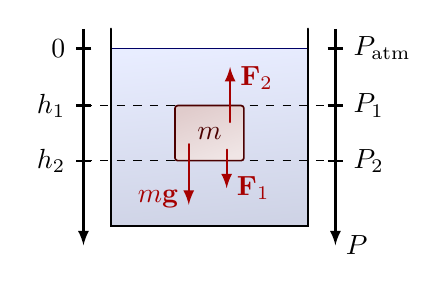
\begin{tikzpicture}
			\def\H{2.5}      % container height
			\def\W{2.5}      % container width
			\def\h{0.9*\H}   % water level height
			\def\my{0.33*\H} % mass y position
			\def\mh{0.28*\H} % mass height
			\def\mw{0.35*\H} % mass width
			
			% CONTAINER
			\draw[water] (-\W/2,0) rectangle++ (\W,\h); %,rounded corners=2
			\draw[thick,line cap=round] (-\W/2,\H) |-++ (\W,-\H) --++ (0,\H);
			
			% MASS
			\draw[dashed]
			(-0.64*\W,\my) -- (0.64*\W,\my)
			(-0.64*\W,\my+\mh) -- (0.64*\W,\my+\mh);
			\draw[mass] (-\mw/2,\my) rectangle++ (\mw,\mh) node[midway] {$m$};
			\draw[force] (0.30*\mw,\my+0.7*\mh) --++ (0,\mh) node[below=4,right=0] {$\vbF_2$};
			\draw[force] (0.25*\mw,\my+0.2*\mh) --++ (0,-0.7*\mh) node[right=0] {$\vbF_1$};
			\draw[force] (-0.3*\mw,\my+0.3*\mh) --++ (0,-1.1*\mh) node[above=2,left=0] {$m\vb{g}$};
			
			% AXIS depth
			\draw[->,thick]
			(-0.64*\W,\H) --++ (0,-1.1*\H);
			\tick{-0.64*\W,\h}{0} node[left] {$0$};
			\tick{-0.64*\W,\my+\mh}{0} node[left] {$h_1$};
			\tick{-0.64*\W,\my}{0} node[left] {$h_2$};
			
			% AXIS pressure
			\draw[->,thick]
			(0.64*\W,\H) --++ (0,-1.1*\H) node[right] {$P$};
			\tick{0.64*\W,\h}{180} node[right] {$P_\mathrm{atm}$};
			\tick{0.64*\W,\my+\mh}{180} node[right] {$P_1$};
			\tick{0.64*\W,\my}{180} node[right] {$P_2$};
			
		\end{tikzpicture}
	\end{center}
	
	E' importante notare che la forza di Archimede si deve ritenere \textbf{applicata al centro di massa}, pertanto oltre alla spinta verso l'alto, nel caso di corpi estesi, si deve pensare anche ad un \textbf{momento risultante}.
	\begin{center}
		\textcolor{red}{inserire grafici}
	\end{center}
	
	
	\subsection{Liquido in rotazione}
	Andiamo a considerare un elemento \(dm\) di liquido e analiziamo le forze in gioco ponendoci nel sistema di riferimento non ineraziale del liquido rotante: 
	\begin{enumerate}
		\item Chiaramente la forza peso: \(\boldsymbol{dmg}\);
		\item Compiendo una traiettoria circolare è soggetto ad una forza centripeta: \(dm\omega^2R = \boldsymbol{\rho dV\omega^2 R}\);
		\item Infine una forza di pressione che va ad equilibrare le altre due: \(\boldsymbol{dF_{P}}\)
	\end{enumerate}
	L'elemento \(dm\) è quindi soggetto a due forze di volume (conservative) e a una forza di pressione. Essendo soggetto a forze conservative possiamo scrivere l'espressione della sua energia potenziale come
	\begin{align*}
		dW = \overrightarrow{F} \cdot d\vec{s} =& (dm \vec{g} - dm \omega^2 \vec{r}) \cdot \boldsymbol{d\vec{s}}\\
		   									   =& dmg\boldsymbol{dz} - dm \omega^2(x+y)\boldsymbol{dxdy}
	\end{align*} 
	\begin{minipage}{0.5\textwidth}
		ponendo lo zero di energia potenziale a terra possiamo ottenere l'espressione di quest'ultima:
		\[ 
		E_{p} = mgz - \frac{1}{2}m\omega ^2(x^2 + y^2)
		\]
		o espressa in unità di massa
		\[ 
		E_{p,m} = gz - \frac{1}{2}\omega ^2(x^2 + y^2)
		\]
		da cui possiamo ottenere l'espressione della coordinata \(z\) in funzione di \(x,y\):
		\begin{equation}
			\viola{z = h +\frac{\omega ^2}{2g}(x^2 +y^2)}
		\end{equation}
		equazione di un \textbf{paraboloide di rotazione}
	\end{minipage}
	\begin{minipage}{0.5\textwidth}
		\begin{center}
			\tdplotsetmaincoords{60}{110}
			\begin{tikzpicture}[tdplot_main_coords,scale=2.0]
				\pgfmathsetmacro{\tini}{0.5*pi}
				\pgfmathsetmacro{\tfin}{1.85*pi}
				\pgfmathsetmacro{\tend}{2.5*pi}
				%%% Coordinate axis
				\draw[thick,->] (0,0,0) -- (1.5,0,0) node [below left] {\footnotesize$x$};
				\draw[dashed] (0,0,0) -- (-1.25,0,0);
				\draw[thick,->] (0,0,0) -- (0,1.5,0) node [right] {\footnotesize$y$};
				\draw[dashed] (0,0,0) -- (0,-1.25,0);
				% The curves slicing the surface
				\draw[mydarkblue,thick,opacity=0.5] plot[domain=-1:1,smooth,variable=\t] ({\t},0,{\t*\t}); 
				\draw[mydarkblue,thick,opacity=0.5] plot[domain=-1:1,smooth,variable=\t] (0,{\t},{\t*\t}); 
				% El paraboloid (for z = constant)
				\foreach \altura in {0.0125,0.025,...,1.0}{
					\pgfmathparse{sqrt(\altura)}
					\pgfmathsetmacro{\radio}{\pgfmathresult}
					\draw[myblue,thick,opacity=0.5] plot[domain=\tini:\tfin,smooth,variable=\t] ({\radio*cos(\t r)},{\radio*sin(\t r)},{\altura}); 
				}
				% Circunference bounding the surface (above, first part)
				\draw[mydarkblue,thick,opacity=0.75] plot[domain=pi:1.75*pi,smooth,variable=\t] ({cos(\t r)},{sin(\t r)},{1.0}); 
				% last part of the z axis
				\draw[thick,->] (0,0,0) -- (0,0,1.75) node [above] {\footnotesize$z$};	
				\foreach \altura in {0.0125,0.025,...,1.0}{
					\pgfmathparse{sqrt(\altura)}
					\pgfmathsetmacro{\radio}{\pgfmathresult}
					\draw[myblue,thick,opacity=0.5] plot[domain=\tfin:\tend,smooth,variable=\t] ({\radio*cos(\t r)},{\radio*sin(\t r)},{\altura}); 
				}
				% Circunference bounding the surface (above, last part)
				\draw[mydarkblue,thick,opacity=0.75] plot[domain=-0.25*pi:pi,smooth,variable=\t] ({cos(\t r)},{sin(\t r)},{1.0}); 
			\end{tikzpicture}
		\end{center}
	\end{minipage}
	
	\vspace{0.3cm}
	Andiamo ora studiare lo stesso caso ma in un sistema di riferimento inerziale. In questo caso l'elemento di liquido non  è più in quiete, la risultante delle forze su di esso dovrà dare un termine centripeto. La condizione di equilibrio è soddisfatta solamente lungo la direzione verticale e, come sappiamo dalla \ref{pressione}, vale

	\begin{align*}
			&\overrightarrow{F}_{V,z} + \overrightarrow{F}_{p,z} = 0 \\
			& dm g + p(z)dS - p(z+dz)dS = 0 \quad  \to \quad dmg - p(dz)dS = 0\\
			& dmg - \frac{\partial p}{\partial z}dzdxdy = 0 \\
			& dmg - \frac{\partial p}{\partial z}dV = 0  \quad \to \quad \rho dV g -  \frac{\partial p}{\partial z}dV = 0 \\
	\end{align*}
	\[ 
	\boxed{\rho g = \frac{\partial p}{\partial z}}
	\]
	Per le forze radiali invece non sono soddisfatte le condizioni di equilibrio (e ricordando che sono forze centripete):
	\begin{align*}
		dF_{r} =& p(r)dS - p(r+dr)dS \\
			   =& - \frac{\partial p}{\partial r}drdS \\
			   =& - \frac{\partial p}{\partial r}dV \\
		-dm \omega^2 r =& - \frac{\partial p}{\partial r}dV \\
		-\rho dV \omega^2 r =& - \frac{\partial p}{\partial r}dV \\
	\end{align*}
	\[ 
	\boxed{\rho \omega^2 r =  \frac{\partial p}{\partial r}}
	\]
	dalle due espressioni si ricava quella della pressione in funzione della distanza radiale e verticale:
	\begin{equation}
		p(r,z) = -\rho gz + \frac{1}{2}\rho \omega ^2 r^2 + p(0,0)
	\end{equation}
	dove \(p(0,0) = p_{0} + \rho gh\) e, ricordando che la superficie libera è isobarica, la pressione atmosferica \(p_{0}\) deve equilibrare \(p(r,z)\)
	\[ 
	p_{0} =  -\rho gz + \frac{1}{2}\rho \omega ^2 r^2 + p_{0} + \rho gh
	\]
	e quindi ritroviamo l'espressione di \(z\) di prima
	\[ 
	z = h +\frac{\omega ^2}{2g}(x^2 +y^2)
	\]
	
	\subsection{Moto  di un fluido}
	Durante lo scorrimento tra due elementi di fluiso compare una \textbf{forza di attrito interno} con verso opposto alla velocit relativa tra i due. Sperimentalmente si trova che il modulo della forza d attrito vale 
	\begin{equation}
		dF = \boldsymbol{\eta} dS \frac{dv}{dn}
	\end{equation}
	
	Il coefficiente \(\boldsymbol{\eta}\) indica la \textbf{viscosià del fluido}; nei liquidi decresce all'aumentare della temperatura, nei gas cresce. Chiamiamo \textbf{fluido ideale} o \textbf{non viscoso e incomprimibile} un fluido con \(\eta = 0\) e \(\rho = \) costante.
	(\textcolor{red}{[!] Il concetto di viscosità assume importanza sono nei fluidi in movimento. La condizione di equilibrio statico  \(dv/dn = 0\) non dipende da \(\eta\)[!]}).
	\\
	
	
	\noindent
	La variazione di forma discussa prima è in parte dovuta all'attrito interno. Il contenitore si mette in modo iniziando a trascinare gli elementi di liquido sulle pareti e sul fondo; glie lementi si portano verso l'esterno fino a che non si stabilisce l'equilibrio dinamico.
	
	\paragraph{Descrizioni del moto}
	\begin{center}
		\begin{minipage}{0.49\textwidth}
			\begin{es}{Lagrangiana}
				Prende in esame un elemento di fluido e ne segue il moto dovuto alle varie forze agenti. In sostanza è una descrizione \textbf{analoga a quella di un punto materiale}.
			\end{es}
		\end{minipage}
		\begin{minipage}{0.49\textwidth}
			\begin{es}{Euleriana}
				Si fissa l'attenzione su un punto della massa fluida \(P(x,y,z)\) e si considera la velocità \(v(x,y,z,t)\) dell'elemento fluido che passa in \(P\) all'instante \(t\).
			\end{es}
		\end{minipage}
	\end{center}
	Spesso risulta più comoda la descrizione euleriana soprattuto se consideriamo la \textbf{velocità indipendente dal tempo}. In questo caso scompare la dipendenza dal tempo che sarebbe rimasta nella visuale lagrangiana (dove si segue il moto del punto).
	\begin{center}
		\fboxsep11pt
		\colorbox{yblue}{\begin{minipage}{5.75in}
				\begin{blues}{Regime stazionario}
					La situazione fisica in cui tutti gli elementi di fluido che passano in istanti diversi in \(P\) hanno in quella posizione sempre stessa velocità, è chiamata \textbf{regime stazionario}.
				\end{blues}
		\end{minipage}}
	\end{center}
	
	\paragraph{Tubi di flusso e portata} Si tracciano delle linee orientate le cui tangenti  serovono a descrivere la direzione e la velocità in quel punto. L'insieme di tutte le linee di corrente attraverso una data sezione prende il nome di \textbf{tubo di flusso}.
	
	\vspace{0.8cm}
	\begin{center}
		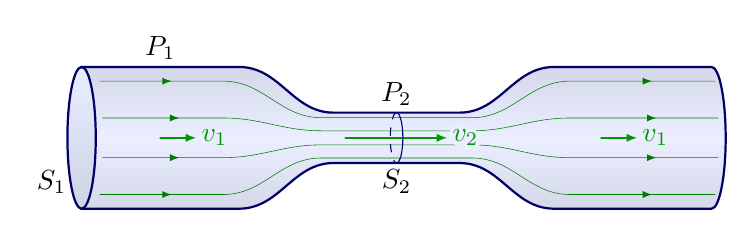
\begin{tikzpicture}
			\def\L{8.0}          % total length
			\def\m{0.20*\L}      % length pipe middle
			\def\l{0.25*\L}      % length pipe outer
			\def\rx{0.08}        % small pipe horizontal radius left
			\def\ry{0.32}        % small pipe vertical radius left
			\def\Rx{0.18}        % big pipe vertical radius right
			\def\Ry{0.90}        % big pipe vertical radius right
			\def\v{1.3}          % velocity magnitude
			\contourlength{1.5pt}
			
			% WATER
			\draw[horizontal water,thick]
			(-\L/2,\Ry) --++ (0,-2*\Ry) coordinate (A1) --++ (\l,0) to[out=0,in=180]
			(-\m/2,-\ry) --++ (\m,0) to[out=0,in=180]
			(\L/2-\l,-\Ry) --++ (\l,0) arc(-90:90:{\Rx} and \Ry) --++ (-\l,0) to[out=180,in=0]
			(\m/2,\ry) --++ (-\m,0) to[out=180,in=0] (-\L/2+\l,\Ry) -- cycle;
			\draw[water,thick]
			(-\L/2,0) ellipse({\Rx} and \Ry);
			\node[above left=2] at (A1) {$S_1$};
			\node[below=-1] at (0,-\ry) {$S_2$};
			
			% VELOCITIES
			\draw[mydarkblue,dashed]
			(0,\ry) arc(90:270:{\rx} and \ry);
			\foreach \fy in {-0.28,-0.8,0.28,0.8}{
				\coordinate (A) at ($(-\L/2,0)+({asin(\fy/1.5)}:{1.5*\Rx} and {1.5*\Ry})$);
				\coordinate (B) at ($({\L/2-\Rx},0)+({asin(\fy/1.5)}:{1.5*\Rx} and {1.5*\Ry})$);
				\draw[vcol!80!black,very thin,postaction={decorate},decoration={markings,
					mark=at position {0.13-0.02*abs(\fy)} with {\arrow{latex}},mark=at position 0.9 with {\arrow{latex}}}]
				(A) -- (-\L/2+0.9*\l,\fy*\Ry) to[out=0,in=180]
				(-0.6*\m,\fy*\ry) -- (0.6*\m,\fy*\ry) to[out=0,in=180] (\L/2-0.9*\l,\fy*\Ry) -- (B);
			}
			\draw[vvec] (-\L/2+0.5*\l,0) --++ (\v*\ry/\Ry,0) node[right=-2] {$v_1$};
			\draw[vvec] ( \L/2-0.7*\l,0) --++ (\v*\ry/\Ry,0) node[right=-2] {$v_1$};
			\draw[vvec] (-0.5*\v,0) --++ (\v,0) node[right=-2] {\contour{watercol!80}{$v_2$}};
			\draw[mydarkblue]
			(0,\ry) arc(90:-90:{\rx} and \ry);
			\node[above=-1] at (-\L/2+0.5*\l,\Ry) {$P_1$};
			\node[above=-1] at (0,\ry) {$P_2$};
		\end{tikzpicture}
	\end{center}
	\vspace{0.8cm}
	
	\begin{center}
		\fboxsep11pt
		\colorbox{yblue}{\begin{minipage}{5.75in}
				\begin{blues}{Portata}
					Viene definita \textbf{portata del tubo di flusso} il volume di fluido che è passato attraverso la sezione in un secondo:
					\begin{equation}
						dq = v dS
					\end{equation}
				\end{blues}
		\end{minipage}}
	\end{center}
	E' importante notare che se \textbf{la configurazione delle linee di corrente è immutabile}, quindi se il fluido è ideale e ci troviamo in condizioni di regime stazionario, \textbf{la portata deve essere la stessa} attraverso qualsiasi sezione. Il fluido in questione infatti, essendo ideale, al variare della sezione non può variare di densità.
	
	
	
	
	\begin{center}
		\fboxsep11pt
		\colorbox{yred}{\begin{minipage}{5.75in}
				\begin{redes}{}
					In regime stazionario, se la densità è costante, è costante la portata di un tubo di flusso infinitesimo:
					\[ 
					vdS = \text{ costante}
					\]
				\end{redes}
		\end{minipage}}
	\end{center}
	
	
		\subsubsection{Teorema di Bernoulli}
		Prendiamo un fluido ideale che scorre in conidzioni di regime stazionario. Il volume \(dV_{1} = S_{1}d\ell_{1}\) che attraversa la sezione \(S_{1}\) nel tempo \(dt\) è uguale a quello \(dV_{2} = S_{2}d\ell_2\) che attraversa nello stesso intervallo la sezionem \(S_{2}\):
		\[ 
		dV_{1} = dV_{2}
		\]
		\begin{center}
			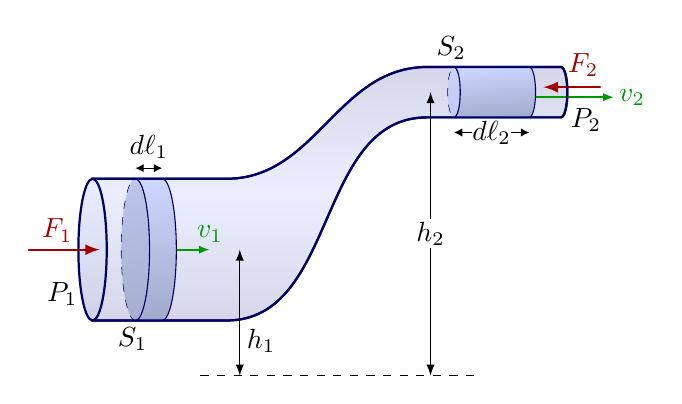
\begin{tikzpicture}
				\def\LL{1.7}          % length pipe left
				\def\LR{1.7}          % length pipe right
				\def\L{3.5*\LL}       % total length
				\def\H{2.0}           % height
				\def\l{\L-\LL-\LR}    % length between pipes
				\def\xL{0.32*\LL}     % position volume left
				\def\xR{\L-0.80*\LR}  % position volume right
				\def\lL{0.2*\LR}      % length volume left
				\def\lR{\lL*\Ry/\ry}  % length volume right
				\def\rx{0.08}         % small pipe horizontal radius left
				\def\ry{0.32}         % small pipe vertical radius left
				\def\Rx{0.18}         % big pipe vertical radius right
				\def\Ry{0.90}         % big pipe vertical radius right
				\def\v{1.0}           % velocity magnitude
				\def\F{0.9}           % force magnitude
				\def\y{(\Ry+0.35*\H)} % height from ground
				
				% WATER
				\draw[horizontal water,thick]
				(0,\Ry) -- (0,-\Ry) coordinate (P1) --++ (\LL,0) to[out=0,in=180]
				(\L-\LR,\H-\ry) -- (\L,\H-\ry) coordinate (P2) arc(-90:90:{\rx} and \ry)
				--++ (-\LR,0)  to[out=180,in=0] (\LL,\Ry) -- cycle;
				\node[above left=2] at (P1) {$P_1$};
				\node[above=-1,right=0] at (P2) {$P_2$};
				
				% VOLUMES
				\draw[vvec] (\xL+\lL+\Rx,0) --++ (\v*1.2*\ry/\Ry,0) node[above=-1] {$v_1$};
				\draw[vvec] (\xR+\lR+\rx,\H-0.2*\ry) --++ (\v,0) node[right=-2] {$v_2$};
				\draw[force] (\L-0.7*\ry+0.8*\F,\H+0.2*\ry) --++ (-0.8*\F,0) node[pos=0.3,above] {$F_2$};
				\draw[dark water,dashed,very thin]
				(\xL,0) ellipse({\Rx} and \Ry)
				(\xR,\H) ellipse({\rx} and \ry);
				\draw[dark water]
				(\xL,\Ry)
				arc(90:-90:{\Rx} and \Ry) coordinate (A1) --++ (\lL,0)
				arc(-90:90:{\Rx} and \Ry) -- cycle;
				\draw[dark water]
				(\xR,\H+\ry) coordinate (A2)
				arc(90:-90:{\rx} and \ry) --++ (\lR,0)
				arc(-90:90:{\rx} and \ry) -- cycle;
				\draw[width]
				(\xL,1.15*\Ry) --++ (\lL,0) node[midway,above] {$d\ell_1$};
				\draw[width]
				(\xR,\H-1.6*\ry) --++ (\lR,0) node[midway,fill=white,inner sep=0] {$d\ell_2$};
				\node[left=1,below=-1] at (A1) {$S_1$};
				\node[left=1,above=-1] at (A2) {$S_2$};
				
				% CONTAINER
				\draw[mydarkblue,thick]
				(0,\Ry) -- (0,-\Ry)  coordinate (A1) --++ (\LL,0) to[out=0,in=180]
				(\L-\LR,\H-\ry) -- (\L,\H-\ry) coordinate (A2) arc(-90:90:{\rx} and \ry)
				--++ (-\LR,0)  to[out=180,in=0] (\LL,\Ry) -- cycle;
				\draw[water,thick]
				(0,0) ellipse({\Rx} and \Ry);
				
				% HEIGHT
				\draw[dashed] (0.23*\L,{-\y}) --++ (0.6*\L,0);
				\draw[<->]
				(1.1*\LL,{-\y}) --++ (0,{\y}) node[pos=0.13,above right=-1] {$h_1$};
				\draw[<->]
				(0.95*\xR,{-\y}) --++ (0,{\H+\y}) node[midway,fill=white,inner sep=1] {$h_2$};
				\draw[force] (0.1*\Ry-\F,0) --++ (\F,0) node[pos=0.4,above=-1] {$F_1$};
				
			\end{tikzpicture}
		\end{center}
		\vspace{0.8cm}
		Andiamo ora a studiare il lavoro delle forze di volume e delle forze di pressione sui due volumi in considerazione:
		
		\begin{center}
			\begin{minipage}{0.49\textwidth}
				\begin{es}{Lavoro forza peso}
					\begin{align*}
						dW_{G} =& =-dE_{p} = \\
							   =& -dm(h_{2} - h_{1})g\\
							   =& -\rho dV(h_{2} - h_{1})g
					\end{align*}
				\end{es}
			\end{minipage}
			\begin{minipage}{0.49\textwidth}
				\begin{es}{Lavoro forze di pressione}
					\begin{align*}
						dW_{P} =& \overrightarrow{F}_{1} \cdot d\vec{\ell}_{1} + \overrightarrow{F}_{2} \cdot d\vec{\ell}_{2} \\
						       =& p_{1} S_{1} d\ell_{1} - p_{2} S_{2} d\ell_{2} \\
						       =& (p_{1} - p_{2})dV
					\end{align*}
				\end{es}
			\end{minipage}
		\end{center}
		Da cui si ricava una variazione di energia cinetica (\(W = \Delta E_{K}\)) pari a
		\[ 
		dE_{K} = dW_{G} + dW_{P} =  (p_{1} - p_{2})dV-\rho dV(h_{2} - h_{1})g
		\]
		\begin{align*}
			dE_{K} =& dW_{G} + dW_{P} \\
			\frac{1}{2}\rho dVv_{2}^2 - \frac{1}{2}\rho dVv_{1}^2	=& (p_{1} - p_{2})dV-\rho dV(h_{2} - h_{1})g \\
		\end{align*}
		\begin{equation}\label{bernoulli}
				\viola{\boxed{p_{1} + \frac{1}{2}\rho v_{1}^2	+ \rho g h_{1} = p_{2} + \frac{1}{2}\rho v_{2}^2	+ \rho g h_{2}}}
		\end{equation}
		\begin{center}
			\fboxsep11pt
			\colorbox{yred}{\begin{minipage}{5.75in}
					\begin{redes}{Teorema di Bernoulli}
						In un fluido ideale in moto con regime stazionario la somma della: \textbf{pressione}, \textbf{densità di energia cinetica} e della \textbf{densità di energia potenziale} è costante lungo il condotto (lungo qualunque tubo di flusso).
					\end{redes}
			\end{minipage}}
		\end{center}
		Notare che dalla legge della dinamica appena presentata, si ricavano tutte le leggi della statica precedenti: \textbf{la statica è sempre un caso particolare della dinamica}. Inoltre si rileva che la pressione misurata in un fluido in movimento è sempre minore di quelal misurata in un fluido in quiete.
		
		\subsubsection{Moto laminare}
		Trattiamo ora il moto di \textbf{fluidi reali}, ovvero fludi di cui non si può più apprissimare \(\eta = 0\) e per cui la densità è approssimabile a un valore costante \(\rho \approx \) costante. A velocità \textit{non elevate} il moto è detto \textbf{laminare}: il regime è stazionario con le linee di corrente costanti nel tempo
		\begin{center}
			\begin{minipage}{0.48\textwidth}
				% LAMINAR FLOW LAYERS
				\hspace{0.6cm}
				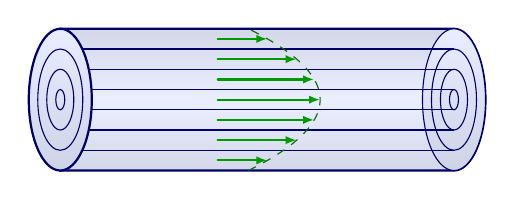
\begin{tikzpicture}
					\def\L{5.0}   % total length
					\def\Rx{0.40} % big pipe vertical radius right
					\def\Ry{0.90} % big pipe vertical radius right
					\def\v{1.3}   % velocity magnitude
					\def\N{3}     % velocity magnitude
					
					% WATER
					\draw[horizontal water,thick]
					(0,\Ry) -- (0,-\Ry)  coordinate (A1) --++ (\L,0) arc(-90:90:{\Rx} and \Ry) -- cycle;
					\draw[water]
					(\L,0) ellipse({\Rx} and \Ry);
					
					\draw[water]
					(0,0) ellipse({\Rx} and \Ry);
					%\draw[horizontal water,line width=0.1] %draw=none
					%  (0,-\Ry) rectangle (\L,\Ry);
					\foreach \i [evaluate={\x=(\i-0.5)/(\N+0.5)}] in {1,...,\N}{
						\draw[mydarkblue] %,line width=0.05
						(0,0) ellipse({\x*\Rx} and \x*\Ry)
						(\L,0) ellipse({\x*\Rx} and \x*\Ry);
						\draw[mydarkblue] %,dashed]  %,line width=0.05
						(0, \x*\Ry) --++ (\L,0)
						(0,-\x*\Ry) --++ (\L,0); %arc(90:-90:{\x*\Rx} and \x*\Ry) --++ (-\L,0);
					}
					%\draw[horizontal water,draw=none]
					%  (0,{-\N/(\N+1)*\Ry}) rectangle (\L,{\N/(\N+1)*\Ry});
					\draw[water,thick]
					(0,0) ellipse({\Rx} and \Ry);
					\foreach \i [evaluate={\x=(\i-0.5)/(\N+0.5)}] in {1,...,\N}{
						\draw[mydarkblue] (0,0) ellipse({\x*\Rx} and \x*\Ry);
					}
					%\draw[mydarkblue,thick]
					%  (0,\Ry) arc(90:-90:{\Rx} and \Ry) coordinate (A1) --++ (\L,0) arc(-90:90:{\Rx} and \Ry) -- cycle;
					\draw[vcol!70!black,dashed,samples=100,smooth,variable=\y,domain=-1:1]
					plot({0.4*\L+\v*(1-0.7*\y*\y)},\y*\Ry);
					\draw[vvec] (0.4*\L,0) --++ (\v,0);
					\foreach \i [evaluate={\y=(\i)/(\N+0.5); \vy=\v*(1-0.7*\y^2);}] in {1,...,\N}{
						\draw[vvec] (0.4*\L, \y*\Ry) --++ (\vy,0);
						\draw[vvec] (0.4*\L,-\y*\Ry) --++ (\vy,0);
					}
					
				\end{tikzpicture}
			\end{minipage}
			\begin{minipage}{0.48\textwidth}
				% PRESSURE
				\hspace{1cm}
				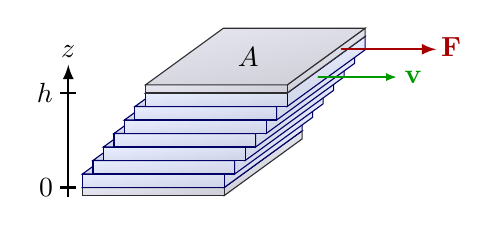
\begin{tikzpicture}[x={(1cm,0)},y={(0.55cm,0.40cm)},z={(0,1cm)}]
					\def\L{1.8}   % cube side
					\def\H{1.2}   % total height
					\def\d{0.8}   % total distance
					\def\N{7}     % number of layers
					\def\t{\H/\N} % layer thickness
					%\draw[dark water] (0,0,0) -- (\L,0,0) -- (\L,\L,0) -- ( 0,\L,0) -- cycle;
					\def\layer#1#2#3#4{
						\draw[#1] (#2+\L,0,#3) --++ (0,\L,0) --++ (0,0,-#4) --++ (0,-\L,0) -- cycle;
						\draw[#1] (#2,0,#3) --++ (\L,0,0) --++ (0,0,-#4) --++ (-\L,0,0) -- cycle;
						\draw[#1] (#2,0,#3) --++ (\L,0,0) --++ (0,\L,0) --++ (-\L,0,0) -- cycle;
					}
					
					\layer{metal}{0}{0}{0.6*\t}
					\foreach \i [evaluate={\x=(\i-1)*\d/(\N-1); \ya=\i*\H/\N; \yb=(\i-1)*\H/\N;}] in {1,...,\N}{
						\layer{water}{\x}{\ya}{\t}
					}
					\layer{metal}{\d}{\H+0.6*\t}{0.6*\t}
					\draw[force] (\L+\d,0.7*\L,\H+0.3*\t) --++ (1.2,0,0) node[above=1,right=-2] {$\vb{F}$};
					\draw[vvec] (\L+\d,0.4*\L,\H-0.5*\t) --++ (1,0,0) node[below=0,right=-1] {$\vb{v}$};
					\node at (\d+0.45*\L,0.5*\L,\H+0.6*\t) {$A$};
					%\draw[width] (0.06*\L,0,0) --++ (0,0,\H) node[midway,fill=white,inner sep=0.5] {$h$};
					\draw[->,thick]
					(-0.1*\L,0,-0.1*\H) --++ (0,0,1.4*\H) node[above=-1] {$z$};
					\tick{-0.1*\L,0,0}{0} node[left=-1] {0};
					\tick{-0.1*\L,0,\H}{0} node[left=-1] {$h$};
					
				\end{tikzpicture}
			\end{minipage}
		\end{center}
		Considerando un condotto lungo \(l\) e di raggio \(R\) si dimostra che la velocità in base alla distanza radiale vale
		\begin{equation}
			\viola{v(r) = \frac{p_{1}-p_{2}}{4\eta l}(R^2-r^2)}
		\end{equation}
		In queste condizioni cambia la formula della portata che diventa
		\[ 
		q = \int_{0}^{R}v(r)2\pi r \ dr
		\]
		da cui si ottiene la \textbf{legge di Hagen-Poiseuille} (valida per raggi molto piccoli)
		\begin{equation}
			q = \frac{\pi R^4}{8\eta}\frac{p_{1} - p_{2}}{l}
		\end{equation}
		dalla quale possiamo trovare il valore della velocità media:
		\begin{equation}
			 \viola{v_{m}= \frac{q}{S} = \frac{\frac{\pi R^4}{8\eta}\frac{p_{1} - p_{2}}{l}}{\pi R^2} = \frac{R^2}{8\eta}\frac{p_{1} - p_{2}}{l}}
		\end{equation}
		Come nel caso di un punto materiale in presenza di attrito radente, per mantenere il flusso di fluido è necessaria una differenza di pressione, ovvero una forza per vincere la resistenza del moto dovuta all'attrito interno.
		
		\subsubsection{Moto turbolento}
		Al crescere del raggio del condotto compaiono vortici nel fluido e si parla di \textbf{moto turbolento o vorticoso}. I vortici sono causati da forti variazioni di velocità ortogonalmente alle linee di corrente, e quindi, a \textbf{notevoli forze di attrito interno} (altre cause sono variazione di forma del condotto...).
		
		Se il condotto è a sezione costante vale la legge sperimentale descritta da Reynolds che ha provato che si ha la transizione da regime laminare a turbolento quando il parametro \(\mathcal{R}\) detto numero di Reynolds super un certo valore critico:
		\[ 
		\mathcal{R} = \frac{\rho v L}{\eta} \qquad  v_{\text{crit}} = \mathcal{R}_{\text{crit}}\frac{\eta}{\rho L}
		\]
		dove \(L\) è la \textbf{lunghezza caratteristica convenzionale} (per tubazioni cilindriche è il diametro).
		
		All'aumentare della differenza di pressione si raggiunge un \textbf{regime di moto stabile in regime turbolento} e si trova che la velocità media si può esprimere come
		\[ 
		v_{m}^2 = 2\frac{L}{k}\frac{\rho }{2} \frac{p_{1} - p_{2}}{l} 
		\]
		Vediamo quindi come il gradiente di pressione \((p_{1}-p_{2}/l)\) sia necessario per mantenere una certa velocità di flusso, più precisamente in regime vorticoso questo è una funzione quadratica della velocità, in regime laminare è una funzione lineare. \\
		
		\noindent
		Consideriamo una sfera immers in un fluido in moto. Se il fluido è ideale si avrà \textbf{completa simmetria delle linee di corrente}, quindi eguale pressione a monte e a valle della sfera che rimarrà ferma; questo risultato è indicato come \textbf{paradosso di D'Alembert}. 
		
		Se invece il fluido è reale si forma una scia vorticosa con pressione a valle maggiore e conseguente applicazione di una forza sulla sfera.
		
		\begin{center}
			\begin{minipage}{0.49\textwidth}
				% LAMINAR FLOW around object
				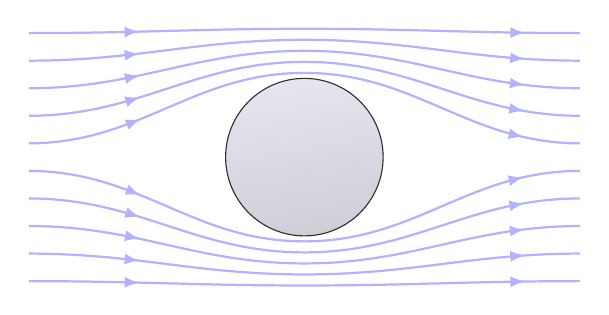
\begin{tikzpicture}
					\def\W{7.0}   % total length
					\def\H{3.5}   % total height
					\def\R{1.0}   % total distance
					\def\N{5}     % number of layers
					\def\t{\H/\N} % layer thickness
					(-0.52*\W,-0.52*\H) rectangle (0.52*\W,0.52*\H);
					\draw[metal]
					(0,0) circle(\R);
					\foreach \s in {-1,1}{
						\foreach \i [evaluate={\fy=\s*(\i-0.5)/\N; \y=\fy*0.5*\H;}] in {1,...,\N}{
							\draw[myblue,thick,postaction={decorate},decoration={markings,
								mark=at position {0.2} with {\arrow{latex}},mark=at position 0.9 with {\arrow{latex}}}]
							(-\W/2,\y) to[out=0,in=180] (0,\s*\R+0.7*\fy) to[out=0,in=180] (\W/2,\y);
						}
					}
				\end{tikzpicture}
				\begin{equation}
					\viola{F_{\text{res}}= 6\pi \eta R v}
				\end{equation}
			\end{minipage}
			\begin{minipage}{0.49\textwidth}
				% TURBULENCE around object
				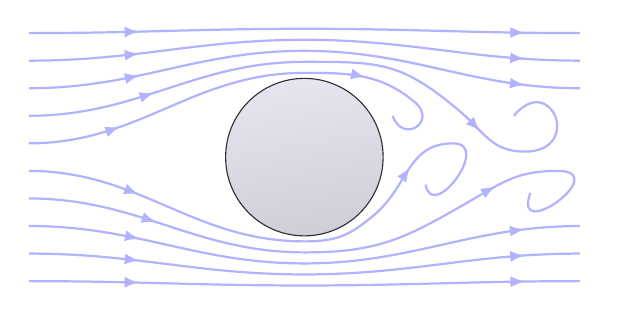
\begin{tikzpicture}
					\def\W{7.0}   % total length
					\def\H{3.5}   % total height
					\def\R{1.0}   % total distance
					\def\N{5}     % number of layers
					\def\t{\H/\N} % layer thickness
					(-0.52*\W,-0.52*\H) rectangle (0.52*\W,0.52*\H);
					\draw[metal]
					(0,0) circle(\R);
					\foreach \s in {-1,1}{
						\foreach \i [evaluate={\fy=\s*(\i-0.5)/\N; \y=\fy*0.5*\H;}] in {3,...,\N}{
							\draw[myblue,thick,postaction={decorate},decoration={markings,
								mark=at position {0.2} with {\arrow{latex}},mark=at position 0.9 with {\arrow{latex}}}]
							(-\W/2,\y) to[out=0,in=180] (0,\s*\R+0.7*\fy) to[out=0,in=180] (\W/2,\y);
						}
					}
					
					%\def\p{node[circle,fill=red,inner sep=0.9] {}} % probe dot
					\draw[myblue,thick,postaction={decorate},decoration={markings,
						mark=at position {0.2} with {\arrow{latex}},mark=at position 0.75 with {\arrow{latex}}}]
					(-\W/2,{1.5/\N*0.5*\H}) to[out=0,in=180] (0,{\R+0.7*1.5/\N}) to[out=0,in=140,looseness=1.2]
					(0.28*\W,0.17*\H) to[out=-40,in=180,looseness=1.1] (0.40*\W,0.02*\H) to[out=0,in=50,looseness=4]
					(0.38*\W,0.15*\H);
					\draw[myblue,thick,postaction={decorate},decoration={markings,
						mark=at position {0.2} with {\arrow{latex}},mark=at position 0.75 with {\arrow{latex}}}]
					(-\W/2,{0.5/\N*0.5*\H}) to[out=0,in=180] (0,{\R+0.7*0.5/\N}) to[out=0,in=140,looseness=1.0]
					(0.20*\W,0.20*\H) to[out=-40,in=-70,looseness=3] (0.16*\W,0.15*\H);
					\draw[myblue,thick,postaction={decorate},decoration={markings,
						mark=at position {0.2} with {\arrow{latex}},mark=at position 0.75 with {\arrow{latex}}}]
					(-\W/2,{-0.5/\N*0.5*\H}) to[out=0,in=180] (0,{-\R-0.7*0.5/\N}) to[out=0,in=-140,looseness=1.1]
					(-40:1.15*\R) to[out=40,in=180,looseness=1.1] (0.27*\W,0.05*\H) to[out=0,in=-80,looseness=2]
					(0.22*\W,-0.10*\H);
					\draw[myblue,thick,postaction={decorate},decoration={markings,
						mark=at position {0.2} with {\arrow{latex}},mark=at position 0.75 with {\arrow{latex}}}]
					(-\W/2,{-1.5/\N*0.5*\H}) to[out=0,in=180] (0,{-\R-0.7*1.5/\N}) to[out=0,in=-150,looseness=1.1]
					(0.30*\W,-0.16*\H) to[out=30,in=180,looseness=1.1] (0.46*\W,-0.05*\H) to[out=0,in=-110,looseness=4]
					(0.41*\W,-0.13*\H);
					
				\end{tikzpicture}
				\begin{equation}
					\viola{F_{\text{res}}= \frac{1}{2}cS\rho v^2}
				\end{equation}
			\end{minipage}
		\end{center}
		Dove la prima è detta \textbf{legge di Stokes} e vale per oggetti di forma sferica, mentre la seconda ha il coefficiente adimensionale \(c\) che dipende dalla forma dell'oggetto (soprattuto la parte posteriore).
			
		
	\subsubsection{Effetto Magnus e Portanza}
	Supponiamo che ora la sfera immersa nel fluido stia anche \textbf{ruotando su se stessa}. Ruotando trasporta per attrito una parte di fluido generando una \textbf{asimmetria} nelle velocità in alto e in basso. In generale la velocità del fluido sarà più alta dove viene trasportato il fluido dalla rotazione (in basso in figura). La differenza di velocità causa una differenza di pressione e quindi una spinta. Questo fenomeno prende il nome di \textbf{effetto Magnus}.
	\begin{center}
		% LAMINAR FLOW around object
		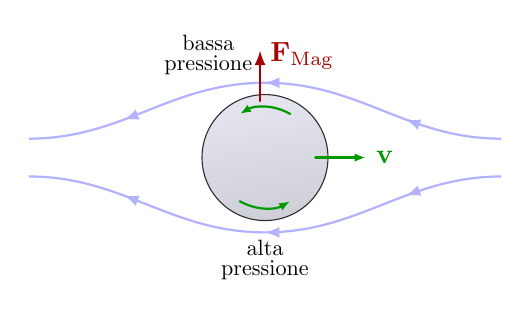
\begin{tikzpicture}
			\def\W{6.0}   % total length
			\def\H{3.1}   % total height
			\def\R{0.8}   % total distance
			
			% WATER
			(-0.52*\W,-0.52*\H) rectangle (0.52*\W,0.52*\H);
			\foreach \s in {-1,1}{
				\draw[myblue,thick,postaction={decorate},decoration={markings,
					mark=at position 0.20 with {\arrow{latex}},
					mark=at position 0.50 with {\arrow{latex}},
					mark=at position 0.80 with {\arrow{latex}}}]
				(\W/2,\s*0.3*\R) to[out=180,in=0] (0,{\s*\R+\s*0.2*(\H/2-\R)}) to[out=180,in=0] (-\W/2,\s*0.3*\R);
			}
			
			% OBJECT
			\draw[metal]
			(0,0) circle(\R);
			\draw[vvec] (0.8*\R,0) --++ (0.8*\R,0) node[right] {$\vb{v}$};
			\draw[vvec] (60:0.8*\R) arc(60:120:0.8*\R);
			\draw[vvec] (-120:0.8*\R) arc(-120:-60:0.8*\R);
			\draw[force] (95:0.9*\R) --++ (0,0.8*\R) node[below=2,right] {$\vb{F}_\mathrm{Mag}$};
			\node[below=-3,scale=0.8,align=center] at (-0.12*\W,0.5*\H) {bassa\\[-1mm]pressione};
			\node[above=-3,scale=0.8,align=center] at (0,-0.5*\H) {alta\\[-1mm]pressione};
			
		\end{tikzpicture}
	\end{center}
	\vspace{2cm}
	Un altro fenomeno importante è la \textbf{portanza}: una spinta verso l'alto dovuta alla differenza di pressioni nelle due parti inferiore e posteriore di un'ala.
	
	Per ricavare un'espressione della forza possiamo passare dall'equazione di Bernoulli. Si hanno i seguenti valori di pressione e velocità:
	\begin{itemize}
		\item \textbf{A monte}: \(p\) e \(v\);
		\item \textbf{Sopra}: \(p_{1}\) e \(v + \Delta v\);
		\item \textbf{Sotto}: \(p_{2}\) e \(v - \Delta v\).
	\end{itemize}
	Deve valere
	\[ 
	p + \frac{1}{2}\rho v^2 = p_{1} + \frac{1}{2}\rho (v+\Delta v)^2= p_{2} + \frac{1}{2}\rho (v-\Delta v)^2
	\]
	da cui 
	\[ 
	p_{2} - p_{1} = 2 \rho v \Delta v
	\]
	che, con una superficie alare \(A\), ci dà
	\begin{equation}
		\viola{F = 2A \rho v \Delta v}
	\end{equation}
	
	
	
	
\newpage
\section{Termodinamica}
\textcolor{red}{Inserire piccolo riassunto pagina 426}\\

\textcolor{red}{Lorem ipsum dolor sit amet, consectetur adipiscing elit, sed do eiusmod tempor incididunt ut labore et dolore magna aliqua. Ut enim ad minim veniam, quis nostrud exercitation ullamco laboris nisi ut aliquip ex ea commodo consequat. Duis aute irure dolor in reprehenderit in voluptate velit esse cillum dolore eu fugiat nulla pariatur. Excepteur sint occaecat cupidatat non proident, sunt in culpa qui officia deserunt mollit anim id est laborum}


\subsection{Termometria}
Chiamiamo \textbf{sistema termodinamico} una porzione del mondo costituita da una oo più parti assimilabile a un sistema continuo macroscopicamente costituito da un numero di elementi pari a \(N_A = 6.0221 \cdot 10^{23}\). L'oggetto di studio saranno le proprietà fisiche macroscopiche e le loro varzioni, \textbf{trasformazioni} del sistema e \textbf{scambi energetici}.

Quando si parlerà di \textbf{ambiente} si intenderà un insieme di una o più parti con cui il sistema termodinamico può interagire. L'ambiente quindi \textbf{contribuisce} in generale \textbf{a determinare le caratteristiche fisiche mascroscopiche del sistema}.

Distinguiamo:
\begin{enumerate}
	\item \textbf{Sistma aperto} se avvengono scambi di energia e materia con l'ambiente;
	\item \textbf{Sistma chiuso} se avvengono solo scambi di energia con l'ambiente;
	\item \textbf{Sistma isolato} se non avvengono scambi con l'ambiente.
\end{enumerate}

\[ 
\viola{\text{{L'insieme (sistema + ambiente) è detto \textbf{universo termodinamico}}}}
\]
\paragraph{Variabili termodinamiche}
Al fine di descrivere il nostro sistema termodinamico viene utilizzato un numero ridotto di variabili termodinamiche, ovvero grandezze fisiche \textbf{direttamente misurabili}. Le distinguiamo in estensive ed intensive:

\begin{center}
\begin{minipage}{0.49\textwidth}
	\begin{es}{Estensive}
		Variabili \textit{additive} che esprimono proprità \textbf{globali} del sistema che dpendono in particolare dalle dimensioni o dall'estensione di quest'ultimo.
		
		\[\viola{\text{Massa}} \qquad \viola{\text{Volume}}\]
		
	\end{es}
\end{minipage}
\begin{minipage}{0.49\textwidth}
	\begin{es}{Intensive}
	Variabili \textit{non additive} che esprimono proprità \textbf{locali} del sistema che possono variare da punto a punto.
	
	\[\viola{\text{Pressione}} \quad \viola{\text{Temperatura}}\quad \viola{\text{Pressione}}\]
	
	\end{es}
\end{minipage}
\end{center}
In base al sistema termodinamico in esame saranno necessarie certe variabili termodinamiche; per esempio per descrivere lo stato di un gas ideale ne sono necessarie 3 \(pVT\) poiché legate dall'equazione di stato \( pV = nRT\) in cui due sono variabili e una dipendente dalle 2.\\

\noindent
\textbf{Osservazione}  La definizione si stato termodinamico è concettualmente diversa da stato meccanico. Uno stato meccanico presuppone la conoscenza di posizione e velocità degli \(n\) corpi interessati, lo stato termodinamico invece, data l'elevato numero di elementi \(n\) non permette ciò, anzi, ad uno stato termodinamico possono essere associti più stati meccanici.

\subsubsection{Equilibrio termico}
\textcolor{red}{Lorem ipsum dolor sit amet, consectetur adipiscing elit, sed do eiusmod tempor incididunt ut labore et dolore magna aliqua. Ut enim ad minim veniam, quis nostrud exercitation ullamco laboris nisi ut aliquip ex ea commodo consequat. Duis aute irure dolor in reprehenderit in voluptate velit esse cillum dolore eu fugiat nulla pariatur. Excepteur sint occaecat cupidatat non proident, sunt in culpa qui officia deserunt mollit anim id est laborum}\\

\noindent
Ora precisiamo il concetto di equilibrio termico. Presi due sistemi A e B con rispettive temperature \(T_A\) e \(T_B\), i sistemi si dicono in \textbf{equilibrio termico} se hanno la stessa temperatura, \(T_A = T_B\)
	\begin{center}
		\fboxsep11pt
		\colorbox{yblue}{\begin{minipage}{5.75in}
				\begin{blues}{Temperatura}
					La temperatura è l'indice dell'equilibrio termico tra due sistemi.
				\end{blues}
		\end{minipage}}
	\end{center}
	
	Per portare due sistemi all'equilibrio termico bisogna porre questi in \textbf{contatto termico} tramite una parete. Se questa parete porta i due sistemi in equilibrio termico, allora prende il nome di  \textbf{parete diatermica}, se no \textbf{parete adiabatica}. \textit{Nella pratica la parete adiabatica e un caso ideale limite}. 
	
	\begin{center}
		\fboxsep11pt
		\colorbox{yblue}{\begin{minipage}{5.75in}
				\begin{blues}{Sistema adiabatico}
					Un sistema è definito adiabatico se è circondato da pareti adiabatiche. Un sistema adiabatico non può essere messo in contatto termico con un'altro sistema o con l'ambiente. \textbf{Una parete è sempre necessaria} per evitare il contatto termico.
				\end{blues}
		\end{minipage}}
	\end{center}
	
	\textit{In generale per il contatto termico non per forza deve entrare in gioco una parete; due solidi a contatto o due fluidi immiscibili non ne hanno bisogno; la parete è necessaria in casi come il contenimento di un gas.}
	
	\begin{center}
		\fboxsep11pt
		\colorbox{yblue}{\begin{minipage}{5.75in}
				\begin{blues}{Definizione operativa di temperatura}
					Per prima cosa occorre identificare un fenomeno fisico che dipenda dalla temperatura \(\theta\) e una grandezza \(X\) che lo caratterizzi. \(X\) è detta \textbf{caratteristica termometrica} e la temperatura funzione di \(X\) è detta \textbf{funzione termometrica} \(\theta(X)\).
					
					Il dispositivo in cui avviene il fenomeno e che fornisce il valore della caratteristica termometrica è indicato come \textbf{termometro}.
				\end{blues}
		\end{minipage}}
	\end{center}

	\begin{center}
	\begin{table}[H]
		\begin{tabular}{@{}lll@{}}
			 \textbf{Termometro}   & \textbf{Fenomeno}   & \textbf{Caratteristica termometrica} \(X\)     \\
			 \textit{a liquido}  & dilatazione termica di un liquido   & lunghezza della colonna di liquido     \\
			 \textit{a resistenza}   & variazione della resistenza elettrica  & resistenza elettrica     \\
			 \textit{a gas a volume costante}   & variazione della pressione  & pressione  \\        
		\end{tabular}
	\end{table}
	\end{center}
	
	
	Nonostante i nostri termometri mostrano una variazione di temperatura lineare, la dipendenza \(\theta(X)\) non lo è (talvolta non è neanche monotona). Nella pratica i termometri vengono utilizzati in intervalli di temperatura nei quali la dipendenza può essere \textbf{approssimata con un andamento lineare} \\
	\[\theta(X) = aX \qquad a \text{ costante}\]\\
	E' essenziale che il sistema di cui noi andiamo a misurare la temperatura sia riproducibile con facilità, per questo si definisce un \textbf{punto fisso}, un valore arbitrario associato al sistema in condizioni di equilibrio facilmente riproducibili. Il punto fisso campione scelto è il \textbf{punto triplo dell'acqua}: stato in cui ghiaccio e acqua e vapor d'acqua saturo sono in equilibrio; a questo stato è stata assegnata la temperatura arbitraria di 
	\[ 
	T_{pt} = \SI{273.16}{\kelvin}
	\]
	Da questa possiamo ricavare la \textbf{temperatura empirica} di un termometro:
	\begin{enumerate}
	\item Si tara il termometro mettendolo in contatto termico con una cella al punto triplo dell'acqua; il termometro, raggiunto l'equilibrio, darà il valore \(X_{pt}\)
	\[ 
	\theta(X_{pt}) = aX_{pt} =  \SI{273.16}{}
	\]
	\item Si pone poi il termometro a contatto con il sistema a temperatura incognita; all'equilibrio il termometro fornirà il valore \(X\)
	\[ 
	\theta(X) = aX = \textcolor{red}{aX_{pt}}\frac{X}{X_{pt}} = \textcolor{red}{\theta(X_{pt})}\frac{X}{X_{pt}} = \textcolor{red}{273.16}\frac{X}{X_{pt}} 
	\]\\
	\begin{equation}\label{temperatura punto triplo}
		\viola{\theta(X) = T  = 273.16\frac{X}{X_{pt}} \SI{ }{[\kelvin]} }
	\end{equation}
	\\
	
	\noindent
	Da cui troviamo anche che la costante \(a\) vale \(a = 273.16/X_{pt}\).
	
	Termometri diversi forniscono sempre letture diverse qando in equilibrio termico con lo stesso stato di un sistema anche se tarati per costruzione al punto triplo dell'acqua (\textit{mio guess: cambierà il tipo di andamento, forse non più lineare}).
	
\end{enumerate}
	\subsubsection{Termometro a gas}
	\begin{center}
		\begin{minipage}{0.49\textwidth}
			\begin{center}
				\textcolor{red}{inserire grafici}
			\end{center}
		\end{minipage}
		\begin{minipage}{0.49\textwidth}
			\begin{center}
				\textcolor{red}{inserire grafici}
			\end{center}
		\end{minipage}
	\end{center}
	Si usa come caratteristica termometrica la pressione:
	
	come prima si misurerà la pressione al punto triplo
	\[ 
	T_{pt} = Cp_{pt}
	\]
	dalla quale ricaviamo la temperatura (\textcolor{red}{[!] non è una definizione accurata [!]})
	\[ 
	T = T_{pt}\frac{p}{p_{pt}} = 273.16\frac{p}{p_{pt}}\SI{}{\kelvin}
	\]
	Come si può vedere dal grafico diminuendo la pressione nel bulbo le temperature dei gas tendono ad assumere valori uguali. Quindi posso dire che la \textbf{pressione} è una \textbf{buona caratteristica temometrica} solo quando è \textbf{bassa}. Quindi il termometro a gas è un buono strumento solo quando il gas è in \textbf{condizioni ideali}.
	
	\[ 
	T = T_{pt}\frac{p}{p_{pt}} = \left(\SI{273.16}{\kelvin}\right)\lim_{p\to 0}\left(\frac{p}{p_{pt}}\right)
	\]
	
	\subsubsection{Dilatazione termica}
	Il volume di un corpo, a pressione costante, aumenta al crescere della temperatura. Presa una sbarra di lunghezza \(L\) a temperatura \(T\) dopo una variazione di temperatura \(\Delta T\) si ha
	\[ 
	L +\Delta L = L + \alpha L\Delta T
	\]
	\[ 
	\viola{\frac{\Delta L}{L} = \alpha \Delta T}
	\]
	con \(\alpha\) coefficiente di dilatazione lineare medio della sostanza. Nel caso di un oggetto isotropo, per la dilatazine volumica si ha
	\[ 
	V + \Delta V = \left(L_1L_2L_3\right) + \left(\alpha L_1 \Delta T\right)\left(\alpha L_2 \Delta T\right)\left(\alpha L_3 \Delta T\right) = V + V(\alpha \Delta T)^3 \approx V + V(3\alpha \Delta T)
	\]
	\[ 
	\viola{\frac{\Delta V}{V} = 3\alpha \Delta T}
	\]
	
	
	\subsection{Esperimenti di Joule}
	Joule condusse una serie di esperimenti sugli\textbf{ effetti termici del lavoro meccanico} (attraverso un mulinello, una resistenza, un pistone, dei blocchi strofinati). Nelle varie esperienza il sistema costituito dall'acqua e dal dispositivo meccanico o elettrico è racchiuso entro \textbf{pareti adiabatiche}. Il risultato ottenuto è che 
	
	\begin{center}
		il \textbf{lavoro}  speso a parità di massa d'acqua è sempre \textbf{proporzionale alla variazione di temperatura} dell'acqua con la stessa costante di proporzionalità.
		\[ 
		W_{ad} = C\Delta T
		\]
	\end{center}
	In analogi acon la definizione di energia potenziale per le forze conservative, introduciamo il concetto di \textbf{energia interna}, energia che dipende solo dallo stato del sistema (cioè dalle sue coordinate termodinamiche):
	\[ 
	W_{ad} = -\Delta U 
	\]
	\begin{es}{convenzione}
		Se il sistema \textbf{fornisce lavoro all'esterno} il lavoro è assunto \textbf{positivo}, se il sistema \textbf{riceve lavoro} dall'ambiente allora il lavoro è assunto \textbf{negativo}.
	\end{es}
	Lo stesso incremento di temperatura è ottenibile senza compiere lavoro meccanico mediante uno \textbf{scambio di calore}, per esempio immergendo un corpo più caldo. Possiamo ottenere lo stesso cambiamento dello stato termodinamico dell'acqua, segnalato dalla stessa variazaione di temparatura per il quale il sistema va ad aumentare la sua energia interna secondo
	\[ 
	Q = \Delta U
	\]
	dove \(Q\) rappresenta il calore scambiato senza lavoro esterno. Da questa otteniamo che 
	\[ 
	Q = \Delta U = -W
	\]
	\begin{equation}\label{Mayer}
		Q = -W_{ad}
	\end{equation}
	Esiste quindi un particolare scambio di energia che non comporta movimenti macroscopici al quale si dà il nome di \textbf{scambio di calore}.
	
	
	\begin{center}
		\fboxsep11pt
		\colorbox{yred}{\begin{minipage}{5.75in}
				\begin{redes}{}
					\subsubsection{Primo principio della termodinamica}
					Se il sistema compie una trasformazione da uno stato A ad uno stato B, scambiando \textbf{calore} e \textbf{lavoro} con l'ambiente, \(Q\) e \(W\) \textbf{dipendono dalla particolare trasformazione} che congiunge i due stati termodinamici mentre \textbf{la differenza \(Q-W\) risulta indipendente} dalla trasformazione.\\
					
					Si può quindi scrivere che la differenza di energia interna 
					\[ 
					U_B - U_A = \Delta U 
					\]
					è uguale alla differenza \(Q-W\):
					\begin{equation}\label{primoprincipio}
						\Delta U = Q -W
					\end{equation}
				\end{redes}
		\end{minipage}}
	\end{center}
	\begin{center}
		\textcolor{red}{inserire grafici}
	\end{center}
	
	\subsubsection{Energia interna}
	Esiste quindi una funzione di stato \textbf{energia interna} le cui variazioni misurano gli scambi di energia con l'esterno durante una trasformazione. Quando si fornisce energia a un sistema questa resta immagazzinata sotto forma di energia interna e può essere poi riutilizzata.
	
	Da notare che l'energia interna non indica l'energia cinetica del sistema, o la sua energia potenziale, bensì energià legata a \textbf{proprietà interne del sistema} come moto molecolare o forze intermolecolari, infatti lo scambio di quest'energia  può avvenire non solo tramite lavoro, ma anche sotto forma di \textbf{scambio di calore}, riconducibile a fenomeni meccanici microscopici.\\
	
	\noindent
	Spesso è utile considerare trasformazioni con variazioni infinitesime del tipo
	\[ 
	dQ = dU + dW
	\]
	dove però \(\boldsymbol{dU}\) è un \textbf{differenziale esatto} perché come abbiamo detto prima la differenza di energia interna è indipendente dalla trasformazione, e \(\boldsymbol{dQ}\) e \(\boldsymbol{dW}\) non sono differenziali esatti poiché questi dipendono da \textit{come si è svolta la trasformazione} e quindi non posso essere espressi come differenza dei valori di una funzione di stato.
	
	\subsection{Trasformazioni termodinamiche}
	I valori di calore e lavoro \(Q\) e \(W\) possono essere calcolati direttamente solo in casi specifici se si conoscono le loro espressioni analitiche dal momento che cambiano con la trasformazione.  Se conosciamo le espressioni di \(\Delta U,Q,W\) in funzione delle coordiante termodinamiche 
	\[ 
	\Delta U = Q -W
	\]
	diventa un'eqwuazione che lega le coordinate termodinamiche durante la trasformazione, quindi diventa \textbf{l'equazione della trasformazione}.\\
	
	\noindent
	Prima di distinguere tre tipi di trasformazioni facciamo qualche osservazione.
	\begin{es}{1. corpi a contatto}
		Prendiamo due corpi a temperature \(T_1\) e \(T_2\) i poniamoli in contatto termico in un contenitore adiabatico. Tra di essi avviene uno scambio di calore fino a che raggiungono l'equilibrio termico. Durante il processo c'è sempre una differenza di temperatura finita, quindi durante la trasformazione \textbf{non c'è mai equilibrio termico}.
	\end{es}
	\begin{es}{2. attrito}
		Preso un cormpo con velocità inizial \(v\) frenato da una forza d'attrito. L'energia cinetica diminuisce e contemporaneamente la temperatura delle superfici a contatto, del corpo e del piano, aumenta. Anche se assumessimo che questo processo avvenga in un tempo molto breve così da poter essere pensato adiabatico, alla fine i corpi cederebbero calore all'ambiente raggiungendo l'equilibrio termico. \\
		
		Quindi nella prima fase non c'è equilibrio meccanico: \(W = -\Delta U = \Delta E_k\), l'energia cinetica decresce quindi l'energia interna cresce. Nella seconda fase invece non c'è equilibrio termico: \(\Delta U = Q\) dove \(Q\) è ceduto all'ambiente quindi \(U\) decresce. Durante il processo quindi \textbf{tutti gli stati intermedi sono di non equilibrio}.
	\end{es}
	
	
	\begin{enumerate}
		\item \textbf{Trasformazioni adiabatiche}: una qualsiasi trasformazione in cui \(Q = 0\) (si ottiene per trasformazioni veloci) e quindi \(\Delta U = - W\). Il sistema non scambia calore con l'ambiente, ossia è \textbf{isolato termicamente}. Sperimentalmente si ottengono le condizioni adiabatiche chiudendo il sistema in un contenitore con pareti adiabatiche. Proprio per questo isolamento il sistema \textbf{non può raggiungere l'equilibrio termico}.
		\item \textbf{Trasformazioni reversibili}: avvengono attraverso stati di eqwuilibrio e in assenza di qualsiasi forza dissipativa. Sono utili perché possono essere arrestate in qualunque stato intermedio e se ne può invertire il verso variando di poco le condizioni esterne.
		\item \textbf{Trasformazioni irreversibili}: avvengono attraverso stati di non equilibrio e/o in presenza di forze dissipative.
	\end{enumerate}
	
	\begin{es}{3. equilibrio}
		Prendiamo una vasca d'acqua con all'interno un contenitore di gas. Le pareti del contenitore sono diatermiche quindi il gas è in equilibrio termico a temperatura costante \(T\). Si può espandere lentamente il contenitore muovendo una parete con una forza che sia sempre uguale e contraria a quella di pressione così da ottenere anche l'equilibrio meccanico. \\
		
		In questo caso tutti gli stati intermedi si possono considerare di equilibrio. Ciò può avvenire solo se si opera una trasformazione \textbf{quasi-statica}, ovvero: prima di procedere a una trasformazione infinitesima di stato si attende il ristabilirsi dell'equilibrio nella nuova condizione.
		(\textcolor{red}{[!] La lentezza delle trasformazioni è condizione solo necessaria e non sufficiente. Vediamo come nel caso 1 si otterrebbero sempre stati intermedi di non equilibrio [!]})
	\end{es}
	
	
	\subsection{Calorimetria}
	Abbiamo visto dal primo teorema della termodinamiche che lo scambio di calore \(Q\) comporta una variazione di energia interna \(\Delta U\) e uno scambio di lavoro \(W\) secondo la legge
	\[ 
	\Delta U = Q -W
	\]
	Per semplicità andremo a studiare scambi di calore tra corpi solidi o liquidi andando a trascurare eventuali dilatazioni e di conseguenza il lavoro meccanico. \\
	
	\noindent
	In un contenitore adiabatico poniamo due corpi a temperature \(T_1\) e \(T_2\) a contatto  in modo che cedano calore \(Q\) fino ad arrivare all'equilibrio termico \(T_e\). Ognuno dei due corpi avrà una variazione della temperatura \(T_{e} - T_i\). 
	Il sistema non scambia lavoro o calore con l'ambiente pertanto l'energia interna resta costante. Andando ad analizzare le energie interne ai due corpi, dovendo essere \(\Delta U = \Delta U_1 + \Delta U_2 = 0\) abbiamo \(\Delta U_1 = -\Delta U_2\); inoltre poiché non è stato compiuto un lavoro meccanico varrà \(Q_1 = -Q_2\): \textbf{il calore ceduto dal corpo è uguale in modulo a quello assorbito dall'acqua}.
	
	
	Dalle misure si trova che esiste (nel limite di piccole variazioni di temperatura) \textbf{proporzionalità} tra il \textbf{calore scambiato} da un corpo, la \textbf{massa} del corpo stesso e la \textbf{variazione di temperatura}:
	\[ 
	Q = m \textcolor{red}{c}(T_f - T_i)
	\]
	dove \(\textcolor{red}{c}\) è il calore specifico caratteristico del corpo (osserviamo che il calore \(Q\) è una grandezza estensiva mentre il calore specivico \(c\) intensiva).
	
	Poiché deve valere \(Q_1 = -Q_2\) vale
	\[ 
	m_1 c_1(T_e - T_1) = -m_2 c_2(T_e - T_2)
	\]
	dalla quale note 3 su 4 variabili si può ricavare la quarta. Nel caso in cui non si possa assumere che il calore specifico sia praticamente costante bisogna scrivere
	\begin{equation}
		\viola{Q = \int dQ = m \int_{T_i}^{T_{f}}c(T)dT}
	\end{equation}
	
	
	\subsubsection{Calore specifico}
	\begin{center}
		\fboxsep11pt
		\colorbox{yblue}{\begin{minipage}{5.75in}
				\begin{blues}{Calore specifico}
					Il calore specifico rappresenta il calore che occorre per scambiare con l'unità di massa di una data sostanza a temperatura \(T\) per farne variare la temperatura di \(\SI{1}{\kelvin}\).
					
					Il calore specifico è una grandezza intensiva caratteristica della sostanza.
				\end{blues}
		\end{minipage}}
	\end{center}
	\begin{center}
		\fboxsep11pt
		\colorbox{yblue}{\begin{minipage}{5.75in}
				\begin{blues}{Capacità termica}
					La capacità termica rappresenta il \textbf{calore da scambiare}  per farne variare la temperatura di \(\SI{1}{\kelvin}\).
					\[ 
					C = mc
					\]
				\end{blues}
		\end{minipage}}
	\end{center}
	Per variazioni infinitesime
	\[ 
	dQ  =mc dT \quad \to \quad c = \frac{1}{m}\frac{dQ}{dT}
	\]
	Spesso si preferisce far riferimento al calore scambiato daun certo numero di moli di sostanza, pertanto si definisce   anche il \textbf{calore specifico molare}
	\[ 
	c = \frac{1}{n}\frac{dQ}{dT}
	\]
	\begin{es}{precisazioni}
	 E' però necessaria una precisaziione riguardo le definizioni di calore specifico. Quando la trasformazione avviene in assenza di lavoro scambiato con l'ambiente \(dW = 0\) e \(dQ = dU\) prt cui
	 \begin{equation}
	 	c  = \frac{1}{m}\frac{dU}{dT} \qquad c  = \frac{1}{n}\frac{dU}{dT}
	 \end{equation}
	 equazioni che valgono solo quando il lavoro è nullo. Se però è compiuto lavoro esterno il calore scambiato dipende dalla trasformazione e è possibile definire diversi calori specifici per una stessa sostanza.
	\end{es}
	\subsubsection{Misura del calore specifico}
	Si può effettuare la amisura del calore specifiico di un corpo tramite il \textbf{calorimetro di Regnault}. In un contenitore adiabatico si ha un recipiente pieno d'acqua a temperatura \(T_2\) con immerso un termometro e un agitatore. Si immerge quindi un corpo a temperatura \(T_1 > T_2\) e di calore specifico incognito \(c_x\). Raggiunto l'equilibrio a temperatura \(T_e\) il bilancio dei calori scambiati in modulo sarà
	\[ 
	m_xc_x(T_1 - T_e) = (C_1 + C_2)(T_e - T_2)
	\]
	dove il primo termine è il calore ceduto dal corpo e il secondo il calore assorbito dal calorimetro.
	\[ 
	c_x = \frac{(C_1 + C_2)(T_e - T_2)}{m_x(T_1 - T_e)}
	\]
	Naturalmente la misura non potrà essere più precida dell'1\% in quanto è impossibile ottenere un perfetto isolamento termico, inoltre la capacità termica del termometro deve essere adeguatamente piccola  in modo da minimizzare lo scambio di calore tra corpo e termometro.
	
	
	\begin{center}
		\textcolor{red}{temp di Debye e legge di Dulong-Petit}
	\end{center}
	
	\subsubsection{Processi isotermi: cambiamenti di fase}
	Si osserva che i cambiamenti di fase sono accompagnati da scambi di calore, più precisamente si tratta di quantità di calore \(\boldsymbol{\lambda}\) ben definite dette  \textbf{calori latenti}. Il calore richiesto per il cambiamento di fase da un corpo di massa \(m\) è 
	\begin{equation}\label{calorelatente}
	\viola{	Q = m\lambda}
	\end{equation}
	La caratteristica importante dei cambiamenti di fase è di essere trasformazioni \textbf{praticamente reversibili}.
	(\textcolor{red}{[!] Il calore latente non ha un valore fisso. Per esempio nel caso dell'evaporazione è funzione della temperatura[!]}).
	
	\subsubsection{Sorgenti di calore}
	\begin{center}
		\fboxsep11pt
		\colorbox{yblue}{\begin{minipage}{5.75in}
				\begin{blues}{Sorgente di calore}
					Si definisce \textbf{sorgente di calore} un corpo con capacità termica praticamente infinita e quindi con la proprietà di poter scambiare calore restando a temperatura costante
				\end{blues}
		\end{minipage}}
	\end{center}
	Grandi masse d'acqua o aria possono essere considerate sorgenti di calore; corpi meno massivi lo possono essere per tempi molto brevi.\\
	
	\noindent
	Proprio per la loro caratteristica di rimanere a temperatura costante, se un corpo è messo a contatto con una sorgente e la differenza di temperatura è finita, \textbf{non può esserci equilibrio termico} durante lo scambio. Può esserci l'equilibrio solo se si mantiene il corpo a contatto con la sorgente abbastanza a lungo (oppure se la differenza di temperatura durante lo scambio è infinitesima).
	
	
	\subsection{Trasmissione del calore}
	
	\subsubsection{Conduzione}
	Prendiamo un corpo esteso in cui la temperatura non sia uniforme e tracciamo le \textbf{superfici isoterme} dove la funzione \(T(x,y,z) = \text{cost}\), diciamo che la superficie \(S_1\) ha temperatura \(T_1\) e così via. 
	
	Se \(dS\) è un elemento della superficie isoterma, il calore che fluisce attraverso \(dS\) nel tempo \(dt\) è 
	\begin{equation}\label{fourier calore}
		\viola{dQ = -\boldsymbol{k} \frac{dT}{dn}dS dt}
	\end{equation}
	\(\boldsymbol{k}\) è la \textbf{conduttività termica} del materiale e dipende dal materiale e dalla temperatura (dipendenza marcata nei metalli dove \(k\) cresce al decrescere della temperatura). Invece essendo \(\frac{dT}{dn}\) il \textbf{gradiente di temperatura} ortogonale a \(dS\) diretto verso temperature crescenti, il \(\boldsymbol{-}\) davanti a tutto indica che il flusso di calore è opposto al verso del gradiente di temperatura:\\
	
	\noindent
	definiamo \(J_U\) il \textbf{flusso di calore per unità di superficie} 
	\[ 
	J_U \equiv \frac{\Delta Q}{\Delta S \Delta t} = - k \frac{dT}{dn}
	\]
	che in forma vettoriale si può scrivere
	\begin{equation}
		\viola{\overrightarrow{J}_U = -k \overrightarrow{\nabla}T}
	\end{equation}
	
	\noindent
	Vediamo come usare in pratica la \ref{fourier calore}: consideriamo una parete piana indefinita \textbf{diatermica} di spessore \(s\) posta tra due ambienti a temperature \(T_1\) e \(T_2\). Andiamo ad analizzare una sezione della parete superficie \(dS\) in \(x\) attraverso la quale viene fornito il calore \(dQ_1\) alla massa \(dm\); intanto \(dm\) attraverso \(dS\) in \(x + dx\) cede il calore \(dQ_2\). Gli scambi di calore saranno quindi:
	\[ 
	dQ_1 = -k \left(\frac{\partial T}{\partial x}\right)_x dS dt
	\]
	\[ 
	dQ_2 = -k \left(\frac{\partial T}{\partial x}\right)_{x+dx} dS dt 
	\]
	che tramite uno sviluppo di Taylor al primo membro
	\[ 
	\textcolor{gray}{f(x) = f(x_0) + f'(x)(x-x_0)}
	\]
	\begin{align*}
		\left(\frac{\partial T}{\partial x}\right)_{x+dx} =& \left(\frac{\partial T}{\partial (x+dx)}\right)_{x+dx} + \left(\frac{\partial^2 T}{\partial (x + dx)^2}\right)_{x+dx}(x - x +dx) \\
		=& \left(\frac{\partial T}{\partial x}\right)_x + \left(\frac{\partial^2 T}{\partial x^2}\right)_{x}dx
	\end{align*}
	
	\[ 
	\to dQ_2 = -k\left[\left(\frac{\partial T}{\partial x}\right)_x + \left(\frac{\partial^2 T}{\partial x^2}\right)_{x}\right]dxdSdt
	\]
	Complessivamente \(dm\) assorbe il calore \(dQ_1\) da sinistra e cede \(dQ_2\) a destra, per cui assorbe 
	\[ 
	dQ_1 - dQ_2  = k\frac{\partial^2 T}{\partial x^2}_{x}dSdx dt
	\]
	quindi ricordando che per variazioni infinitesime vale
	\[ 
	dQ = dmcdT = \rho dS dx c dT
	\]
	troviamo che 
	\[ 
	k\frac{\partial^2 T}{\partial x^2}_{x}\textcolor{red}{dSdx} dt = \rho  \textcolor{red}{dSdx} c dT
	\]
	ottenendo la legge che regola la variazione di temperatura in funzione del tempo e della posizione della parete (con \(T(x=0) = T_1\) e \(T(x = s) = T_2\))
	\begin{equation}
		\viola{\frac{\partial^2 T}{\partial x^2} = \rho \frac{c}{k} \frac{\partial T}{\partial t}}
	\end{equation}
	\begin{es}{A regime}
		Arrivati alla temperatura di regime e una volta che la temperatura di ciascun punto ha raggiunto un valore stazionario \textbf{costante nel tempo} si annulla la derivata temporale e di conseguenza anche la derivata seconda spaziale:
		\[ 
		\frac{\partial T}{\partial t} = 0 \quad \Rightarrow \quad \frac{\partial^2 T}{\partial x^2} = 0\quad \Rightarrow \quad T(x) = \alpha + \beta x
		\]
		imponendo
		\begin{align*}
			&T(0) = T_1 = \alpha  \\
			&T(s) = T_2 = \alpha + \beta s = T_1 + \beta s
		\end{align*}
		\[ 
		\beta = \frac{T_2 - T_1}{s} 
		\]
		possiamo riscrivere l'andamento della temperatura come
		\[ 
		T(x) = T_1 - \frac{T_1 - T_2}{s}x \qquad |\overrightarrow{\nabla}T |= \frac{T_1 - T_2}{s}
		\]
		che mostra come la temperatura decresca linearmente partendo dal valore massimo (\(x=0\)) \(T_1\) fino al valore minimo (\(x=s\)) \(T_2\). \\
		
		Prima avevamo definito il il calore che flusice attraverso una superficie \(dS\) in un tempo \(dt\) come
		\[ 
		dQ = -k\frac{dT}{dn}dS dt
		\]
		dalla quale ricaviamo che, nel nostro caso, attraverso \(dS\) flusice il calore 
		\[ 
		Q = k\frac{T_1 - T_2}{s}St
		\](\textcolor{red}{[!] In \textbf{regime stazionario} il calore che entra nella parete dal lato ad alta temperatura è uguale al calore che esce dal lato a assa temperatura. \textbf{C'è solo flusso di energia} e nessuna cessione alla parete [!]}).
	\end{es}
	
	\paragraph{Equazione di continuità} Presa una superficie orientata \(\Sigma\) in un mezzo non in equilibrio termico di volume \(V\), in assenza di sorgenti di calore in \(V\) il calore che esce per unità di tempo da \(V\) attraverso \(\Sigma\) è uguale a meno la variazione per unità di tempo del calore contenuto in \(V\):
	
	\[ 
	\int_{\Sigma} \overrightarrow{J}_U \cdot \hat{n} dS = -\frac{d}{dt}\int_V \boldsymbol{q} dV = - \int_V \frac{\partial q}{\partial t} dV
	\]
	ocn \(\boldsymbol{q}\) energia termica per unità di volume. \\
	
	\noindent
	Se andiamo a riscriverla in forma differenziale otteniamo
	\[ 
	\overrightarrow{J}_U \cdot \hat{n}dS = - \frac{\partial q}{\partial t} dV
	\]
	e quindi come per i fluidi ()
	\begin{equation}
	\viola{	\frac{\partial q}{\partial t} + \overrightarrow{\nabla} \cdot \overrightarrow{J}_U  = 0 }
	\end{equation}
	
	\begin{center}
		\textcolor{red}{inserire grafici}
	\end{center}
	
	
	\subsubsection{Convezione}
	La connduzione termica nei fluidi è difficile da osservare perché in essi avviene un altro fenomeno di trasmissione del calore: la convezione.
	
	Riscaldando un fluido la parte più vicina alla sorgente di calore si scalda prima dilatandosi. Le parti di fluido più calde risentono quindi di una spinta di Archimede maggiore e tendono a spostarsi verso l'alto generando correnti ascensionali che fanno avvicinare le parti di fluido più fredde alla sorgente. 
	
	\subsubsection{Irraggiamento}
	L'energia emessa sotto forma di onde elettromagnetiche in unità di tempo è descritta dalla \textbf{legge di Stefan-Boltzman} come
	\begin{equation}\label{stefan boltzman}
		\viola{\varepsilon = \boldsymbol{\sigma e}T^4}
	\end{equation}
	dove \(\boldsymbol{\sigma} = 5.67\cdot 10^{-8}\SI{}{\frac{\joule}{\second\meter^2\kelvin^4}}\) è una costante universale ed \(\boldsymbol{e}\) è l'\textbf{emissività} che varia tra \(0\) e \(1\): \(0\) per le pareti riflettenti, \(1\) per le cosiddette superfici nere. Una superficie nera assorbe tutta l'energia che incide su di essa.
	
	\subsubsection{Calore tra solido e fluido}
	La trasmissione del calore tra un corpo solido a temperatura \(T\) e un fluido a temperatura \(T_0 < T\) messi a contatto tramite una superficie \(S\) è descritta dalla \textbf{legge di Newton}
	\begin{equation}
		\viola{Q = \boldsymbol{h}(T-T_0)St}
	\end{equation}
	dove \(\boldsymbol{h}\) è la \textbf{conducibilità termica esterna}
	
	\subsection{Gas ideali e reali}
	\subsubsection{Legge isoterma di Boyle}
	\subsubsection{Legge isocora di Volta-Gay Lussac}
	\subsubsection{Legge di Avogadro}
	
	\subsection{Trasformazioni  di un gas}
	\subsubsection{Calore e energia interna del gas ideale}
	\subsubsection{Relazione di Mayer}
	
	\subsubsection{Trasformazioni adiabatiche}
	Il gas è racchiuso da pareti adiabariche e può scambiare solo lavoro con l'ambiente (tramite una parete mobile).
	 
	\begin{align*}
		Q = 0 \quad \Rightarrow \quad W_{AB} =& -\Delta U \\
											 =& -nc_{V} T
	\end{align*}
	
	\[ 
	pV = nRT \quad \Rightarrow \quad nT = \frac{pV}{R}
	\]
	Presa una trasformazione dal punto \(A\) al punot \(B\) si avrà quindi
	\begin{align*}
		W_{AB} =& nc_{V}(T_{A} - T_{B}) = c_{v}\frac{(p_{A}V_{A} - p_{b}V_{B})}{R} \\
			   =& \frac{1}{\gamma -1}(p_{A}V_{A} - p_{b}V_{B})
	\end{align*}
	con 
	\[ 
	\boxed{c_{P} - c_{V} = R}
	\]
	
	\subsubsection{Trasformazioni isoterme}
	\subsubsection{Trasformazioni isocore}
	\subsubsection{Trasformazioni isobare}
	
	
\end{document}




